\section*{Appendix Table of Contents}
\begin{itemize}
    \item \textbf{Appendix \ref{app:extended_related_work}: Extended Related Work}
    \item \textbf{Appendix \ref{apendix:corpus_details}: Corpus Details}
    \begin{itemize}
        \item \ref{sec:appendix_task_detail} Task Metadata and Scale
        \item \ref{sec:appendix_algo_details} Algorithm and Architecture Distribution
        \item \ref{sec:appendix_agent_benchmark} Agent Evaluation Benchmark
        \item \ref{sec:trajectory_sampling} Trajectory Sampling and Intermediate States
    \end{itemize}
    \item \textbf{Appendix \ref{appendix:detailed_exp_result}: Detailed Experiment Result}
    \begin{itemize}
        \item \ref{app:fine_grained_performance} Fine-grained Performance on Prediction Corpus
        \item \ref{app:trajectory_variance} Analysis of Pair Source and Trajectory Variance
        \item \ref{app:ai4s_bench} Detailed Performance Metrics of \ours on AI4Science Benchmarks
        \item \ref{app:search_efficiency} Search Efficiency Analysis of \ours
        \item \ref{app:fidelity_analysis} Decision Fidelity and Reliability in Local Iterations
        \item \ref{app:ablation_k} Ablation Study on Top $k$ Selection
        \item \ref{app:license} Licensing and Artifact Usage
        \item \ref{app:compute} Computational Infrastructure and Budget
        \item \ref{app:packages} Software Dependencies and Metric Implementation
    \end{itemize}
    \item \textbf{Appendix \ref{appendix:case_studies}: Detailed Qualitative Analysis}
    \begin{itemize}
        \item \ref{app:case_bias} Case I: Overcoming Complexity Bias
        \item \ref{app:case_domain} Case II: Domain Fit over Architectural Sophistication
        \item \ref{app:case_report} Case III: Sample of the Verbal Data Report
        \item \ref{app:case_instruction} Case IV: Sample of the Task Instruction ($I$)
    \end{itemize}
    \item \textbf{Appendix \ref{appendix:prompt_templates}: Prompt Templates}
\end{itemize}
\vspace{1em}


\section{Extended Related Work}
\label{app:extended_related_work}

This section expands upon the brief literature review in Section~\ref{sec:related-work}, providing a detailed taxonomy of LLM-based autonomous agents and the theoretical underpinnings of world models in the code domain.

\paragraph{LLM-based Agents for Scientific Discovery}
LLMs with strong reasoning capabilities~\cite{qiao-etal-2023-reasoning} are increasingly serving as core controllers for autonomous agents in scientific discovery~\cite{gu2024largelanguagemodelsconstructing,chen2025ai4researchsurveyartificialintelligence}, extending to specialized machine research domains~\cite{toledo2025airesearchagentsmachine, Wen-lin2025}.
Beyond the digital realm, agents are transforming laboratory research~\cite{liu2025alphagomomentmodelarchitecture, li2025mlrcopilotautonomousmachinelearning, Yuxuan2025, schmidgall2025agentlaboratoryusingllm} and complex data analytics~\cite{sun2025agenticdataagenticdataanalytics, zhang2025deepanalyzeagenticlargelanguage}.
Prominent systems now autonomously propose hypotheses~\cite{chai2025scimastergeneralpurposescientificai, yu2025alpharesearchacceleratingnewalgorithm, internagentteam2025internagentagentscientist, novikov2025alphaevolvecodingagentscientific} and conduct closed-loop experiments~\cite{gottweis2025aicoscientist, lange2025shinkaevolveopenendedsampleefficientprogram, yuan2025dolphinmovingclosedloopautoresearch, yu2025researchtownsimulatorhumanresearch, WOS:001446914500004}, highlighting the trend of ``AI Scientists'' operating in open-ended exploration loops.

Narrowing down to the machine learning domain, the ecosystem is highly diversified.
One stream of research focuses on managing the end-to-end workflow, ranging from autonomous frameworks~\cite{nam2025mlestarmachinelearningengineering, yang2025rdagentllmagentframeworkautonomous, qiao2025scalinggeneralistdataanalyticagents, Ze-xi2025} to engineering pipelines~\cite{Fang2025, chi2024selatreesearchenhancedllm, DOI:10.3724/2096-7004.di.2024.0005}.
Another stream, driven by benchmarks like MLE-bench~\cite{chan2025mlebenchevaluatingmachinelearning, huang2024mlagentbenchevaluatinglanguageagents} and broader evaluation suites~\cite{zhang2025mlrcbenchlanguageagentssolve, jing2024dsbench, zhang2024benchmarking, Nathani2025}, focuses on competitive problem-solving through knowledge-guided reasoning~\cite{luo2025executableknowledgegraphsreplicating, ou2025automindadaptiveknowledgeableagent} and evolutionary optimization~\cite{du2025automlgennavigatingfinegrainedoptimization, guo2024dsagentautomateddatascience, li2025fmagent, liu2025mlmasteraiforaiintegrationexploration}.

Additionally, general-purpose platforms and optimization frameworks offer the foundational tooling and multi-agent architectures required for scalable research~\cite{wang2025openhandsopenplatformai, jiang2025aideaidrivenexplorationspace, hong2024datainterpreterllmagent, qiang2025mledojointeractiveenvironmentsempowering, wang2025configurablemultiagentframeworkscalable}.
However, to mitigate the significant computational overhead of the generation-execution-feedback loop inherent in these systems, recent approaches explore utilizing internal priors to estimate feasibility and prune redundant steps, thereby accelerating optimization~\cite{kulibaba2025kompeteaiacceleratedautonomousmultiagent, trirat2025automlagentmultiagentllmframework, Zhang2024, Astorga2024}.


\paragraph{Operational Details of Agent Baselines}

As introduced in Section~\ref{sec:agent_paradigm}, we take two representative agent frameworks that operate under the \textbf{Generate-Execute-Feedback} paradigm as examples. Here we provide their detailed mechanisms:

\begin{itemize}
    \item \textbf{AIDE:} AIDE~\citep{jiang2025aideaidrivenexplorationspace} is an LLM-based agent that frames machine learning engineering as a code optimization problem.
    It structures the trial-and-error process as a tree search in the solution space, reusing and refining promising code candidates.
    This method effectively trades computational resources for enhanced performance.
    Specifically, AIDE first generates initial code $C_0$ based on instruction $I$.
    The code is executed by training on dataset $D$ to obtain results. Subsequently, AIDE iteratively derives new code $C_1, C_2, \dots, C_t$ based on the feedback.

    \item \textbf{AutoMind:} Building upon the AIDE framework, AutoMind~\citep{ou2025automindadaptiveknowledgeableagent} further integrates a curated expert knowledge base and a self-adaptive coding strategy.
    While retaining the tree search structure, it grounds the agent in domain expertise and dynamically tailors code generation to task complexity.
    This approach aims to reduce invalid attempts by improving the quality of the initial draft and subsequent refinements.
\end{itemize}


\paragraph{World Models and Execution-Free Evaluation}
The concept of World Models originates from model-based reinforcement learning, where agents learn to simulate the environment's transition dynamics to plan actions without expensive trial-and-error~\cite{Ding2025, hafner2024masteringdiversedomainsworld, feng2025webworldmodels, wong2023wordmodelsworldmodels, li2025wordworldlargelanguage}.
Our work adapts this concept to the code generation domain, addressing the ``Execution Bottleneck'' inherent in the agentic loops described above.

Recent research enables models to internalize the execution process, predicting test outcomes~\cite{Hora2024predictingtestresultswithoutexecution, faircodegenteam2025cwmopenweightsllmresearch,wei2025swerladvancingllmreasoning} or assessing logic consistency directly~\cite{li2025codeiocondensingreasoningpatterns, Changshu2024codemind}.
This capability is rigorously evaluated on reasoning-centric benchmarks~\cite{wei2025equibenchbenchmarkinglargelanguage, gu2024cruxevalbenchmarkcodereasoning, jain2024livecodebenchholisticcontaminationfree}.
Unlike traditional benchmarks that may allow for rote memorization, these tasks require models to transcend statistical pattern matching and develop a deep semantic understanding of algorithmic states and control flows~\cite{chen2025scalingagentlearningexperience, sun2025zerosearchincentivizesearchcapability, akhauri2025regressionlanguagemodelscode, Chen2025reval}, serving as the foundational capability for our proposed framework.
Aligning with OpenAI's Level 4 ``Innovators''~\cite{metz2024openai, zhang2025innogymbenchmarkinginnovationpotential}, this empowers agents to drive innovation by leveraging internal world models to proactively prune vast hypothesis spaces, shifting the paradigm from ensuring syntactic correctness to optimizing for semantic success.
This transition resonates with the broader Data-Centric AI movement~\cite{zha2023datacentricartificialintelligencesurvey, cabrera2025machinelearningsystemssurvey}, moving beyond model architecture to focus on the quality of evaluative signals.
Specifically, our framework incorporates rationale-based preference optimization~\cite{Just2024datacentrichuman} and rigorous dataset construction criteria~\cite{Shen2024towardsdatacentricrlhf} to ensure that the ``implicit world model'' is grounded in data-specific realities rather than abstract heuristics~\cite{tschalzev2024datacentricperspectiveevaluatingmachine}.



\section{Corpus Details}
\label{apendix:corpus_details}

To support the reproducibility of our analysis and provide a comprehensive view of the solution space, we provide detailed metadata for the corpus.


\subsection{Task Metadata and Scale}
\label{sec:appendix_task_detail}
Table~\ref{tab:appendix_task_details_part1} outlines the specific characteristics of each of the 26 tasks, including the domain, machine learning paradigm, data size, and the scale of the constructed evaluation set.


\subsection{Algorithm and Architecture Distribution}
\label{sec:appendix_algo_details} % 给这一小节一个标签，方便引用

As shown in Figure~\ref{fig:algo_diversity_sunburst} and Table~\ref{tab:appendix_algo_dist_part1}, the solutions range from traditional statistical methods to advanced deep learning architectures, ensuring that our analysis is evaluated against a heterogeneous solution manifold.

% \begin{longtable}{
%     >{\raggedright\arraybackslash}p{0.18\linewidth} 
%     >{\raggedright\arraybackslash}p{0.36\linewidth} 
%     >{\raggedright\arraybackslash}p{0.15\linewidth} 
%     r r r
% }
% % --- 第一页表头 ---
%     \toprule
%     \textbf{Task Name} & \textbf{Task Description} & \textbf{ML Paradigm} & \textbf{Size} & \textbf{Sol} & \textbf{Pair} \\
%     \midrule
%     \endfirsthead
    
%     % --- 续页表头 ---
%     \multicolumn{6}{c}{{\bfseries \tablename\ \thetable{} -- continued from previous page}} \\
%     \toprule
%     \textbf{Task Name} & \textbf{Task Description} & \textbf{ML Paradigm} & \textbf{Size} & \textbf{Sol} & \textbf{Pair} \\
%     \midrule
%     \endhead
    
%     % --- 页脚 (非最后一页) ---
%     \bottomrule
%     \multicolumn{6}{r}{{Continued on next page}} \\
%     \endfoot
    
%     % --- 最后一页页脚 (包含 Caption 和间距) ---
%     \bottomrule
%     \addlinespace[1em] % 增加垂直间距
%     \caption{Detailed metadata for all 26 tasks in the Prediction Corpus. The table details the problem definition, ML paradigm, data size, and evaluation scale.} 
%     \label{tab:appendix_task_details} \\
%     \endlastfoot

%     % ================= Computer Vision =================
%     \multicolumn{6}{l}{\cellcolor{gray!15}\textbf{\textit{Computer Vision Domain}}} \\
%     \midrule
%     APTOS 2019 Blindness & Detect diabetic retinopathy severity from retinal fundus images. & Img Class. (Multi-class) & 8.1G & 50 & 1,225 \\ \addlinespace
    
%     Dog Breed Identification & Identify dog breed from photos (120 categories). & Img Class. (Multi-class) & 369M & 3 & 3 \\ \addlinespace
    
%     Leaf Classification & Classify 99 plant species based on leaf shape features. & Img Class. (Multi-class) & 30M & 17 & 136 \\ \addlinespace
    
%     MLSP 2013 Birds & Identify bird species from audio spectrograms. & Img Class. (Multi-label) & 634M & 50 & 1,221 \\ \addlinespace
    
%     Plant Pathology 2020 & Distinguish healthy vs. diseased apple leaves. & Img Class. (Multi-class) & 387M & 6 & 15 \\ \addlinespace
    
%     Statoil Iceberg Classifier & Distinguish icebergs from ships in radar imagery. & Img Class. (Binary) & 205M & 50 & 1,223 \\ \addlinespace
    
%     ICML 2013 Whale & Identify individual Right Whales by callosity patterns. & Img Class. (Multi-class) & 377M & 24 & 275 \\ \addlinespace
    
%     TGS Salt Identification & Segment salt deposits from seismic images. & Segmentation (Pixel-level) & 59M & 44 & 880 \\ \addlinespace
    
%     Denoising Dirty Docs & Restore clean text from noisy scanned documents. & Img Restoration (Reg.) & 97M & 45 & 974 \\ \addlinespace
    
%     % ================= NLP =================
%     \multicolumn{6}{l}{\cellcolor{gray!15}\textbf{\textit{Natural Language Processing Domain}}} \\
%     \midrule
%     Detecting Insults & Detect insulting language in social commentary. & Text Class. (Binary) & 2M & 27 & 350 \\ \addlinespace
    
%     Jigsaw Toxic Comment & Classify comments into 6 toxicity types (toxic, severe, etc.). & Text Class. (Multi-label) & 129M & 5 & 10 \\ \addlinespace
    
%     Spooky Author ID & Identify author (Poe, Shelley, Lovecraft) of excerpts. & Text Class. (Multi-class) & 3.2M & 50 & 1,220 \\ \addlinespace
    
%     Random Acts of Pizza & Predict success of free pizza requests on Reddit. & Text Class. (Binary) & 21M & 50 & 1,225 \\ \addlinespace
    
%     US Patent Matching & Determine semantic similarity between patent phrases. & Matching (Class.) & 316M & 50 & 1,223 \\ \addlinespace
    
%     Google QUEST & Predict 30 subjective attributes (e.g., helpfulness) for Q\&A. & Multi-output (Reg.) & 14M & 50 & 1,224 \\ \addlinespace
    
%     Tweet Sentiment Extract & Extract substring supporting the sentiment label. & Seq. Labeling (Extract) & 3.3M & 21 & 210 \\ \addlinespace
    
%     LMSYS Chatbot Arena & Predict human preference between two LLM responses. & Ranking (Preference) & 176M & 50 & 1,220 \\ \addlinespace
    
%     Automated Essay Scoring & Automatically grade student essays on a numeric scale. & Regression (Ordinal) & 35M & 20 & 190 \\ \addlinespace
    
%     % ================= Data Science Domain =================
%     \multicolumn{6}{l}{\cellcolor{gray!15}\textbf{\textit{Data Science Domain}}} \\
%     \midrule
%     NYC Taxi Fare & Predict taxi fare from coordinates and time. & Tabular (Regression) & 5.3G & 30 & 429 \\ \addlinespace
    
%     PetFinder Pawpularity & Predict popularity score of pet profile photos. & Regression (Hybrid) & 1.0G & 30 & 239 \\ \addlinespace
    
%     NOMAD Conductors & Predict formation energy of aluminum-gallium oxides. & Regression (Scientific) & 25M & 3 & 3 \\ \addlinespace
    
%     Stanford COVID Vaccine & Predict degradation rates of mRNA vaccine sequences. & Regression (Bio) & 14M & 50 & 1,222 \\ \addlinespace
    
%     Tabular Playground & Predict forest cover type from cartographic variables. & Tabular (Multi-class) & 526M & 24 & 275 \\ \addlinespace
    
%     Volcanic Eruptions & Predict time to next eruption from seismic sensors. & Time-Series (Reg.) & 15G & 50 & 1,213 \\ \addlinespace
    
%     Ventilator Pressure & Predict airway pressure from control inputs. & Time-Series (Reg.) & 291M & 50 & 1,222 \\ \addlinespace
    
%     TF Speech Recognition & Identify spoken commands from audio clips. & Audio (Multi-class) & 2G & 46 & 1,011 \\ 
    
% \end{longtable}


\begin{table*}
    \centering
    \footnotesize
    
    \begin{tabular}{
        >{\raggedright\arraybackslash}p{0.18\linewidth} 
        >{\raggedright\arraybackslash}p{0.36\linewidth} 
        >{\raggedright\arraybackslash}p{0.15\linewidth} 
        r r r
    }
    \toprule
    \textbf{Task Name} & \textbf{Task Description} & \textbf{ML Paradigm} & \textbf{Size} & \textbf{Sol} & \textbf{Pair} \\
    \midrule

    % ================= Computer Vision =================
    \multicolumn{6}{l}{\cellcolor{gray!15}\textbf{\textit{Computer Vision Domain}}} \\
    \midrule
    APTOS 2019 Blindness & Detect diabetic retinopathy severity from retinal fundus images. & Img Class. (Multi-class) & 8.1G & 50 & 1,225 \\ \addlinespace
    
    Dog Breed Identification & Identify dog breed from photos (120 categories). & Img Class. (Multi-class) & 369M & 3 & 3 \\ \addlinespace
    
    Leaf Classification & Classify 99 plant species based on leaf shape features. & Img Class. (Multi-class) & 30M & 17 & 136 \\ \addlinespace
    
    MLSP 2013 Birds & Identify bird species from audio spectrograms. & Img Class. (Multi-label) & 634M & 50 & 1,221 \\ \addlinespace
    
    Plant Pathology 2020 & Distinguish healthy vs. diseased apple leaves. & Img Class. (Multi-class) & 387M & 6 & 15 \\ \addlinespace
    
    Statoil Iceberg Classifier & Distinguish icebergs from ships in radar imagery. & Img Class. (Binary) & 205M & 50 & 1,223 \\ \addlinespace
    
    ICML 2013 Whale & Identify individual Right Whales by callosity patterns. & Img Class. (Multi-class) & 377M & 24 & 275 \\ \addlinespace
    
    TGS Salt Identification & Segment salt deposits from seismic images. & Segmentation (Pixel-level) & 59M & 44 & 880 \\ \addlinespace
    
    % ================= NLP =================
    \multicolumn{6}{l}{\cellcolor{gray!15}\textbf{\textit{Natural Language Processing Domain}}} \\
    \midrule
    Detecting Insults & Detect insulting language in social commentary. & Text Class. (Binary) & 2M & 27 & 350 \\ \addlinespace

    Jigsaw Toxic Comment & Classify comments into 6 toxicity types (toxic, severe, etc.). & Text Class. (Multi-label) & 129M & 5 & 10 \\ \addlinespace

    Spooky Author ID & Identify author (Poe, Shelley, Lovecraft) of excerpts. & Text Class. (Multi-class) & 3.2M & 50 & 1,220 \\ \addlinespace
    
    Random Acts of Pizza & Predict success of free pizza requests on Reddit. & Text Class. (Binary) & 21M & 50 & 1,225 \\ \addlinespace

    US Patent Matching & Determine semantic similarity between patent phrases. & Matching (Class.) & 316M & 50 & 1,223 \\ \addlinespace

    Denoising Dirty Docs & Restore clean text from noisy scanned documents. & Img Restoration (Reg.) & 97M & 45 & 974 \\ \addlinespace
    
    Google QUEST & Predict 30 subjective attributes (e.g., helpfulness) for Q\&A. & Multi-output (Reg.) & 14M & 50 & 1,224 \\ \addlinespace
    
    Tweet Sentiment Extract & Extract substring supporting the sentiment label. & Seq. Labeling (Extract) & 3.3M & 21 & 210 \\ \addlinespace
    
    LMSYS Chatbot Arena & Predict human preference between two LLM responses. & Ranking (Preference) & 176M & 50 & 1,220 \\ \addlinespace
    
    Automated Essay Scoring & Automatically grade student essays on a numeric scale. & Regression (Ordinal) & 35M & 20 & 190 \\ \addlinespace
    
    % --- 模仿 longtable 的页脚 ---
    \bottomrule
    \multicolumn{6}{r}{\textit{Continued on next page}} \\ % 手动添加这一行
    \end{tabular}

    \caption{Detailed metadata for all 26 tasks in the Prediction Corpus (Part 1 of 2). The table details the problem definition, ML paradigm, data size, and evaluation scale.}
    \label{tab:appendix_task_details_part1}
    
\end{table*}


\begin{table*}[t!]
    \centering
    \footnotesize
    
    \begin{tabular}{
        >{\raggedright\arraybackslash}p{0.18\linewidth} 
        >{\raggedright\arraybackslash}p{0.36\linewidth} 
        >{\raggedright\arraybackslash}p{0.15\linewidth} 
        r r r
    }
    % --- 模仿 longtable 的续页表头 ---
    \multicolumn{6}{c}{{\bfseries \tablename\ \thetable{} -- continued from previous page}} \\
    \toprule
    \textbf{Task Name} & \textbf{Task Description} & \textbf{ML Paradigm} & \textbf{Size} & \textbf{Sol} & \textbf{Pair} \\
    \midrule

    % ================= NLP (Continued) =================
    % 这里是从 Part 1 移过来的 NLP 任务

    % Denoising Dirty Docs & Restore clean text from noisy scanned documents. & Img Restoration (Reg.) & 97M & 45 & 974 \\ \addlinespace
    
    % Google QUEST & Predict 30 subjective attributes (e.g., helpfulness) for Q\&A. & Multi-output (Reg.) & 14M & 50 & 1,224 \\ \addlinespace
    
    % Tweet Sentiment Extract & Extract substring supporting the sentiment label. & Seq. Labeling (Extract) & 3.3M & 21 & 210 \\ \addlinespace
    
    % LMSYS Chatbot Arena & Predict human preference between two LLM responses. & Ranking (Preference) & 176M & 50 & 1,220 \\ \addlinespace
    
    % Automated Essay Scoring & Automatically grade student essays on a numeric scale. & Regression (Ordinal) & 35M & 20 & 190 \\ \addlinespace

    % ================= Data Science Domain =================
    \multicolumn{6}{l}{\cellcolor{gray!15}\textbf{\textit{Data Science Domain}}} \\
    \midrule
    NYC Taxi Fare & Predict taxi fare from coordinates and time. & Tabular (Regression) & 5.3G & 30 & 429 \\ \addlinespace
    
    PetFinder Pawpularity & Predict popularity score of pet profile photos. & Regression (Hybrid) & 1.0G & 30 & 239 \\ \addlinespace
    
    NOMAD Conductors & Predict formation energy of aluminum-gallium oxides. & Regression (Scientific) & 25M & 3 & 3 \\ \addlinespace
    
    Stanford COVID Vaccine & Predict degradation rates of mRNA vaccine sequences. & Regression (Bio) & 14M & 50 & 1,222 \\ \addlinespace
    
    Tabular Playground & Predict forest cover type from cartographic variables. & Tabular (Multi-class) & 526M & 24 & 275 \\ \addlinespace
    
    Volcanic Eruptions & Predict time to next eruption from seismic sensors. & Time-Series (Reg.) & 15G & 50 & 1,213 \\ \addlinespace
    
    Ventilator Pressure & Predict airway pressure from control inputs. & Time-Series (Reg.) & 291M & 50 & 1,222 \\ \addlinespace
    
    TF Speech Recognition & Identify spoken commands from audio clips. & Audio (Multi-class) & 2G & 46 & 1,011 \\ 
    \bottomrule
    \end{tabular}
    
    % 【关键步骤】让表格编号倒退 1
    \addtocounter{table}{-1}
    
    \caption{Detailed metadata for all 26 tasks (Part 2 of 2). Continued from previous page.}
    \label{tab:appendix_task_details_part2}
    
\end{table*}

% \newpage


\subsection{Agent Evaluation Benchmark}
\label{sec:appendix_agent_benchmark}

We curated a specialized benchmark to test the World Model's capability to generalize from seen tasks to unseen scientific problems. As detailed in Table~\ref{tab:agent_benchmark}, this selection covers diverse AI4Science domains including Biology, Physics, Geoscience, Ecology, and Medicine. Note that tasks marked with ``*'' (Aerial Cactus and Histo. Cancer Detect) are \textit{unseen} tasks, meaning they were not used in the main experiments and serve as out-of-distribution evaluations.


% --- 算法表格（详细数据） ---
% \begin{table*}[t!]
%     \centering
%     \footnotesize
    
%     \begin{tabular}{
%         >{\raggedright\arraybackslash\bfseries}p{0.23\linewidth} 
%         >{\raggedright\arraybackslash}p{0.72\linewidth}
%     }
%     \toprule
%     Task Name & Algorithm Composition (Count) \\
%     \midrule

%     % ================= Computer Vision =================
%     \multicolumn{2}{l}{\cellcolor{gray!15}\textbf{\textit{Computer Vision Domain}}} \\
%     \midrule
%     APTOS 2019 Blindness & EfficientNet (10), ResNet (10), Swin Transformer (9), ConvNeXt (9), Vision Transformer (8), DeiT (3), CNN-LSTM (1) \\ \addlinespace
    
%     Dog Breed ID & ConvNeXt-Large (2), ResNet18 (1) \\ \addlinespace
    
%     Leaf Classification & LightGBM (13), Feedforward NN (2), HybridLeafClassifier (1), XGBoost (1) \\ \addlinespace
    
%     MLSP 2013 Birds & Ensemble (12), Dual-Stream Arch (5), Feedforward NN (5), Multi-Modal NN (5), Transformer Enc (5), CNN (5), Random Forest (4), XGBoost (4), Logistic Reg (4), LightGBM (1) \\ \addlinespace
    
%     Plant Pathology & EfficientNet (2), Swin Transformer (2), ResNet (1), Vision Transformer (1) \\ \addlinespace
    
%     Statoil Iceberg & Inverted Bottleneck (5), Vision Trans. (5), ResNet (5), Feedforward NN (5), XGBoost (5), CNN (5), Hybrid CNN-ViT (4), Swin Trans. (4), ConvNeXt (4), Random Forest (3), LightGBM (3), EfficientNet (1), SVM (1) \\ \addlinespace
    
%     ICML Whale Challenge & Wav2Vec2 Feature Extractor (10), CNN (6), XGBoost (4), Gradient Boosting (2), LightGBM (1), Mel Spectrogram (1) \\ \addlinespace
    
%     TGS Salt ID & Ensemble Segmentation (12), EfficientNet (10), U-Net (10), DeepLabV3Plus (4), Vision Transformer (4), Single Seg. Model (2), Swin Trans. (1), ConvNeXt (1) \\ \addlinespace
    
%     Denoising Dirty Docs & Residual Dense Network (10), U-Net (10), Conv Autoencoder (10), Restormer (8), Hybrid CNN-Transformer (6), Simple CNN (1) \\ \addlinespace
    
%     % ================= NLP =================
%     \multicolumn{2}{l}{\cellcolor{gray!15}\textbf{\textit{Natural Language Processing Domain}}} \\
%     \midrule
%     Detecting Insults & DeBERTa (9), Multi-Task DeBERTa-V3 (6), RoBERTa (4), DistilBERT (3), BERT (3), Logistic Regression (2) \\ \addlinespace
    
%     Jigsaw Toxic Comment & RoBERTa (3), DistilBERT (1), DeBERTa (1) \\ \addlinespace
    
%     Spooky Author ID & Knowledge Distillation (4), DeBERTa (4), ELECTRA (4), BERT (4), LSTM (4), XGBoost (4), Ensemble (4), SVM (4), Logistic Reg (4), Random Forest (3), LightGBM (3), Naive Bayes (3), MLP (2), Transformer (2), Hierarchical Trans. (1) \\ \addlinespace
    
%     Random Acts of Pizza & Neural Network (6), SentenceTransformer (4), RoBERTa (4), Knowledge Distillation (4), Multimodal NN (4), BERT (4), DistilBERT (4), Random Forest (4), XGBoost (4), Logistic Reg (4), LightGBM (4), LMs Text Embeddings (4) \\ \addlinespace
    
%     US Patent Matching & Custom NN (5), RoBERTa (5), DeBERTa (5), XGBoost (5), BERT (5), Sentence Trans. (5), Similarity Model (5), Linear Reg (5), LightGBM (5), Stacking Ensemble (2), RandomForest (2), Cross-Attn Hybrid (1) \\ \addlinespace
    
%     Google QUEST & BERT (5), Multi-Task NN (5), MultiModal Trans. (5), Graph Attention (3), Hierarchical Attn (3), MLP (3), Cross-Attn (3), Sentence Trans. (3), DeBERTa (3), RoBERTa (3), XGBoost (3), LightGBM (3), Ridge Reg. (3), ELECTRA (2), Random Forest (2), LSTM (1) \\ \addlinespace
    
%     Tweet Sentiment & RoBERTa-BiLSTM (10), RoBERTa (10), Model Ensemble (1) \\ \addlinespace
    
%     LMSYS Chatbot Arena & RoBERTa (11), XGBoost (8), Logistic Reg. (8), LightGBM (8), MLP Classifier (7), DeBERTa (4), Dual Encoder NN (4) \\ \addlinespace
    
%     Automated Essay Score & Hybrid NN (9), MetaModel NN (5), Stacking Ensemble (3), LightGBM (3) \\ \addlinespace
    
%     % ================= Data Science =================
%     \multicolumn{2}{l}{\cellcolor{gray!15}\textbf{\textit{Data Science Domain}}} \\
%     \midrule
%     NYC Taxi Fare & LightGBM (10), XGBoost (10), Feedforward NN (7), CatBoost (1), Dual-Branch NN (1), Residual NN (1) \\ \addlinespace
    
%     PetFinder Pawpularity & LightGBM (27), Vision Transformer (2), XGBoost (1) \\ \addlinespace
    
%     NOMAD Conductors & XGBoost (2), Random Forest (1) \\ \addlinespace
    
%     Stanford COVID Vac. & Hybrid Architectures (14), Model Ensemble (9), Transformer/GNN (6), Specialized RNA Models (6), Tree Boosters (6), General Baselines (7), LSTM (2) \\ \addlinespace
    
%     Tabular Playground & Multi-Branch NN (11), LightGBM (7), Custom NN (3), TabTransformer (2), Feedforward NN (1) \\ \addlinespace
    
%     Volcanic Eruptions & Tree Boosters (19), MLP/Dense Networks (16), Transformer Variants (6), CNN/Hybrid Architectures (6), Model Ensemble (2), TCN (1) \\ \addlinespace

%     Ventilator Pressure & RNNs (LSTM/GRU) (17), Hybrid Deep Learning (CNN/TCN/Attn) (13), Tree Boosters (10), Transformers (9), Statistical Baseline (1) \\ \addlinespace

%     TF Speech Recognition & Statistical ML (RF/SVM/LR) (21), CNN Architectures (13), Pre-trained Audio Models (Wav2Vec2/WavLM) (8), Transformer (2), MLP (1), Knowledge Distillation (1) \\
    
%     \bottomrule
%     \end{tabular}

%     \caption{Distribution of algorithms and architectures across the corpus. The parenthesized number denotes the count of unique solutions employing that specific method.} 
%     \label{tab:appendix_algo_dist}
    
% \end{table*}


\begin{table*}[t!]
    \centering
    \footnotesize
    
    \begin{tabular}{
        >{\raggedright\arraybackslash\bfseries}p{0.23\linewidth} 
        >{\raggedright\arraybackslash}p{0.72\linewidth}
    }
    \toprule
    Task Name & Algorithm Composition (Count) \\
    \midrule

    % ================= Computer Vision =================
    \multicolumn{2}{l}{\cellcolor{gray!15}\textbf{\textit{Computer Vision Domain}}} \\
    \midrule
    APTOS 2019 Blindness & EfficientNet (10), ResNet (10), Swin Transformer (9), ConvNeXt (9), Vision Transformer (8), DeiT (3), CNN-LSTM (1) \\ \addlinespace
    
    Dog Breed ID & ConvNeXt-Large (2), ResNet18 (1) \\ \addlinespace
    
    Leaf Classification & LightGBM (13), Feedforward NN (2), HybridLeafClassifier (1), XGBoost (1) \\ \addlinespace
    
    MLSP 2013 Birds & Ensemble (12), Dual-Stream Arch (5), Feedforward NN (5), Multi-Modal NN (5), Transformer Enc (5), CNN (5), Random Forest (4), XGBoost (4), Logistic Reg (4), LightGBM (1) \\ \addlinespace
    
    Plant Pathology & EfficientNet (2), Swin Transformer (2), ResNet (1), Vision Transformer (1) \\ \addlinespace
    
    Statoil Iceberg & Inverted Bottleneck (5), Vision Trans. (5), ResNet (5), Feedforward NN (5), XGBoost (5), CNN (5), Hybrid CNN-ViT (4), Swin Trans. (4), ConvNeXt (4), Random Forest (3), LightGBM (3), EfficientNet (1), SVM (1) \\ \addlinespace
    
    ICML Whale Challenge & Wav2Vec2 Feature Extractor (10), CNN (6), XGBoost (4), Gradient Boosting (2), LightGBM (1), Mel Spectrogram (1) \\ \addlinespace
    
    TGS Salt ID & Ensemble Segmentation (12), EfficientNet (10), U-Net (10), DeepLabV3Plus (4), Vision Transformer (4), Single Seg. Model (2), Swin Trans. (1), ConvNeXt (1) \\ \addlinespace
    
    Denoising Dirty Docs & Residual Dense Network (10), U-Net (10), Conv Autoencoder (10), Restormer (8), Hybrid CNN-Transformer (6), Simple CNN (1) \\ 
    
    \bottomrule
    \multicolumn{2}{r}{\textit{Continued on next page}} \\
    \end{tabular}

    \caption{Distribution of algorithms and architectures across the corpus (Part 1 of 2). The table details the algorithm composition for Computer Vision tasks.} 
    \label{tab:appendix_algo_dist_part1}
    
\end{table*}


\begin{table*}[t!]
    \centering
    \footnotesize
    
    \begin{tabular}{
        >{\raggedright\arraybackslash\bfseries}p{0.23\linewidth} 
        >{\raggedright\arraybackslash}p{0.72\linewidth}
    }
    % --- 续页表头 ---
    \multicolumn{2}{c}{{\bfseries \tablename\ \thetable{} -- continued from previous page}} \\
    \toprule
    Task Name & Algorithm Composition (Count) \\
    \midrule

    % ================= NLP =================
    \multicolumn{2}{l}{\cellcolor{gray!15}\textbf{\textit{Natural Language Processing Domain}}} \\
    \midrule
    Detecting Insults & DeBERTa (9), Multi-Task DeBERTa-V3 (6), RoBERTa (4), DistilBERT (3), BERT (3), Logistic Regression (2) \\ \addlinespace
    
    Jigsaw Toxic Comment & RoBERTa (3), DistilBERT (1), DeBERTa (1) \\ \addlinespace
    
    Spooky Author ID & Knowledge Distillation (4), DeBERTa (4), ELECTRA (4), BERT (4), LSTM (4), XGBoost (4), Ensemble (4), SVM (4), Logistic Reg (4), Random Forest (3), LightGBM (3), Naive Bayes (3), MLP (2), Transformer (2), Hierarchical Trans. (1) \\ \addlinespace
    
    Random Acts of Pizza & Neural Network (6), SentenceTransformer (4), RoBERTa (4), Knowledge Distillation (4), Multimodal NN (4), BERT (4), DistilBERT (4), Random Forest (4), XGBoost (4), Logistic Reg (4), LightGBM (4), LMs Text Embeddings (4) \\ \addlinespace
    
    US Patent Matching & Custom NN (5), RoBERTa (5), DeBERTa (5), XGBoost (5), BERT (5), Sentence Trans. (5), Similarity Model (5), Linear Reg (5), LightGBM (5), Stacking Ensemble (2), RandomForest (2), Cross-Attn Hybrid (1) \\ \addlinespace
    
    Google QUEST & BERT (5), Multi-Task NN (5), MultiModal Trans. (5), Graph Attention (3), Hierarchical Attn (3), MLP (3), Cross-Attn (3), Sentence Trans. (3), DeBERTa (3), RoBERTa (3), XGBoost (3), LightGBM (3), Ridge Reg. (3), ELECTRA (2), Random Forest (2), LSTM (1) \\ \addlinespace
    
    Tweet Sentiment & RoBERTa-BiLSTM (10), RoBERTa (10), Model Ensemble (1) \\ \addlinespace
    
    LMSYS Chatbot Arena & RoBERTa (11), XGBoost (8), Logistic Reg. (8), LightGBM (8), MLP Classifier (7), DeBERTa (4), Dual Encoder NN (4) \\ \addlinespace
    
    Automated Essay Score & Hybrid NN (9), MetaModel NN (5), Stacking Ensemble (3), LightGBM (3) \\ \addlinespace
    
    % ================= Data Science =================
    \multicolumn{2}{l}{\cellcolor{gray!15}\textbf{\textit{Data Science Domain}}} \\
    \midrule
    NYC Taxi Fare & LightGBM (10), XGBoost (10), Feedforward NN (7), CatBoost (1), Dual-Branch NN (1), Residual NN (1) \\ \addlinespace
    
    PetFinder Pawpularity & LightGBM (27), Vision Transformer (2), XGBoost (1) \\ \addlinespace
    
    NOMAD Conductors & XGBoost (2), Random Forest (1) \\ \addlinespace
    
    Stanford COVID Vac. & Hybrid Architectures (14), Model Ensemble (9), Transformer/GNN (6), Specialized RNA Models (6), Tree Boosters (6), General Baselines (7), LSTM (2) \\ \addlinespace
    
    Tabular Playground & Multi-Branch NN (11), LightGBM (7), Custom NN (3), TabTransformer (2), Feedforward NN (1) \\ \addlinespace
    
    Volcanic Eruptions & Tree Boosters (19), MLP/Dense Networks (16), Transformer Variants (6), CNN/Hybrid Architectures (6), Model Ensemble (2), TCN (1) \\ \addlinespace

    Ventilator Pressure & RNNs (LSTM/GRU) (17), Hybrid Deep Learning (CNN/TCN/Attn) (13), Tree Boosters (10), Transformers (9), Statistical Baseline (1) \\ \addlinespace

    TF Speech Recognition & Statistical ML (RF/SVM/LR) (21), CNN Architectures (13), Pre-trained Audio Models (Wav2Vec2/WavLM) (8), Transformer (2), MLP (1), Knowledge Distillation (1) \\
    
    \bottomrule
    \end{tabular}

    % 编号回退，保持与 Part 1 相同的 Table 编号
    \addtocounter{table}{-1}
    \caption{Distribution of algorithms and architectures across the corpus (Part 2 of 2). Continued from previous page (NLP and Data Science domains).} 
    \label{tab:appendix_algo_dist_part2}
    
\end{table*}

\begin{table*}
    \centering
    \footnotesize
    
    \begin{tabular}{
        >{\raggedright\arraybackslash\bfseries}p{0.20\linewidth} 
        >{\raggedright\arraybackslash}p{0.38\linewidth} 
        >{\raggedright\arraybackslash}p{0.15\linewidth} 
        l 
        c
    }
    % --- 表头 ---
    \toprule
    Task Name & Task Description & ML Paradigm & Size & Status \\
    \midrule

    % ================= SEEN TASKS =================
    \multicolumn{5}{l}{\cellcolor{gray!15}\textbf{\textit{Seen Tasks (In-Distribution)}}} \\
    \midrule
    Stanford COVID Vaccine & \textit{(Biology)} Predict RNA degradation rates at various locations along RNA sequences to assist in mRNA vaccine stability research. & Regression (Seq) & 14M & \textbf{Seen} \\ \addlinespace

    Ventilator Pressure & \textit{(Physics)} Simulate the pressure of a mechanical ventilator connected to a sedated patient's lung to optimize breathing assistance. & Regression (Time-Series) & 291M & \textbf{Seen} \\ \addlinespace

    Statoil Iceberg & \textit{(Geoscience)} Distinguish between icebergs and ships in satellite radar imagery (SAR) to improve navigation safety. & Classification (Image) & 205M & \textbf{Seen} \\ \addlinespace

    % ================= UNSEEN TASKS =================
    \multicolumn{5}{l}{\cellcolor{gray!15}\textbf{\textit{Unseen Tasks (Out-of-Distribution)}}} \\
    \midrule
    Aerial Cactus Identification* & \textit{(Ecology)} Determine the presence of columnar cacti in high-resolution aerial imagery to track protected species in the desert. & Classification (Image) & 25.4M & \textbf{Unseen} \\ \addlinespace

    Histopathologic Cancer Detection.* & \textit{(Medicine)} Identify metastatic cancer tissue in small image patches taken from larger digital pathology scans. & Classification (Image) & 7.7G & \textbf{Unseen} \\
    
    \bottomrule
    \end{tabular}

    \caption{Agent Evaluation Benchmark. The table details the specific tasks used to evaluate the agent, categorized by their domain and their visibility status (Seen vs. Unseen).}
    \label{tab:agent_benchmark}

\end{table*}

% --- 算法分布图（Sunburst Chart） ---
% 强调这张图的宏观概览作用
\begin{figure*}
    \centering
    % 请确保你的图片路径正确，且为 PDF 格式
    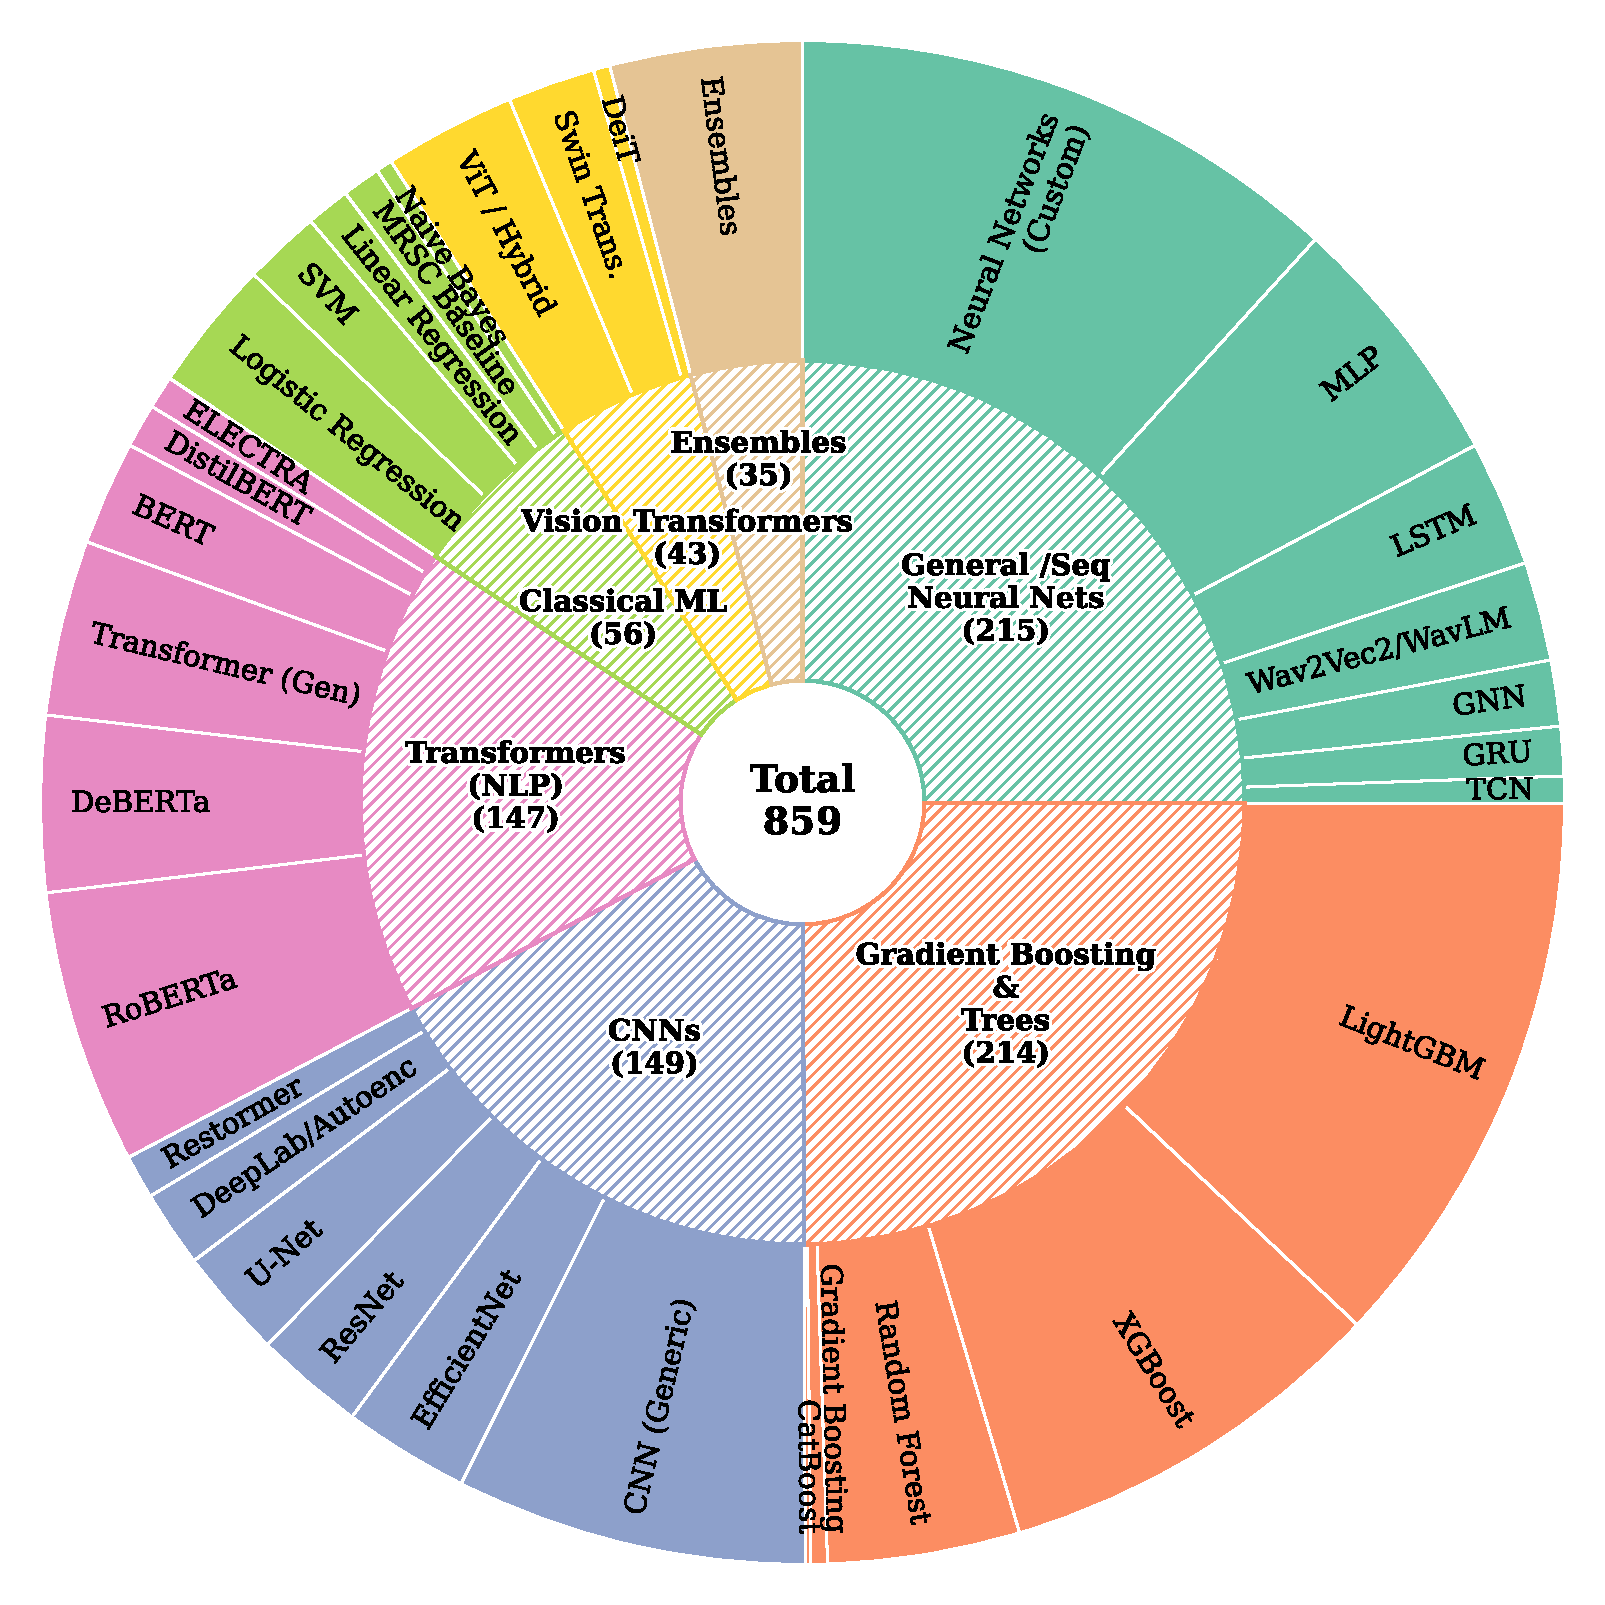
\includegraphics[width=0.8\textwidth]{figures/appendix_algo_distribution_pie.pdf} 
    \caption{Hierarchical distribution of the unique solution architectures in our Prediction Corpus. The chart illustrates the balance achieved across major machine learning paradigms: Gradient Boosting\&Trees, General/Sequential NNs, CNNs, and Transformers. The outer ring details specific model instances, demonstrating the high heterogeneity of the solution space.}
    \label{fig:algo_diversity_sunburst}
\end{figure*}


\subsection{Trajectory Sampling and Intermediate States}
\label{sec:trajectory_sampling}

To clarify the composition of our Preference Corpus, it is important to note that the dataset captures the entire lifecycle of an agent's exploration.
While we filter out syntactically invalid code that crashes, our dataset is rich in logically imperfect intermediate states. 

As shown in Figure \ref{fig:trajectory_tree}, we generate pairs not just from the final best solution, but across the entire valid search path. 
This extensively tests the model's implicit modeling capabilities to distinguish and guide improvements among messy and unfinalized intermediate code states, ensuring the agent moves from working but poor to working and good.

\newsavebox{\myverbbox}
\begin{figure*}
\centering
\begin{lrbox}{\myverbbox}
\begin{minipage}{0.85\textwidth}
\footnotesize
\begin{verbatim}
Root
 |-- Bug (Syntax Error) [Filtered: Handled by Interpreter]
 |    \-- Bug (Runtime Error) [Filtered]
 |         \-- Score: 0.380 (Valid, Intermediate "Half-baked") -> INCLUDED
 |              \-- Score: 0.377 (Valid, Improved) -> INCLUDED
 |                   |-- Score: 0.385 (Valid, Regressed) -> INCLUDED
 |                   |-- Score: 0.377 (Valid, Best-so-far) -> INCLUDED
 |                   \-- Score: 0.383 (Valid, Sub-optimal) -> INCLUDED
\end{verbatim}
\end{minipage}
\end{lrbox}
\fbox{\usebox{\myverbbox}}
\caption{A representative trajectory snippet illustrating our sampling strategy. This extensively tests the model's implicit modeling capabilities to distinguish and guide improvements among messy and unfinalized intermediate code states, ensuring the agent moves from working but poor to working and good.}
\label{fig:trajectory_tree}
\end{figure*}





\section{Detailed Experiment Result}
\label{appendix:detailed_exp_result}

In this section, we provide a comprehensive breakdown of the experimental results, supplementing the main paper with granular performance metrics across individual tasks, domains, and agent architectures.

\subsection{Fine-grained Performance on Prediction Corpus}
\label{app:fine_grained_performance}
Table~\ref{tab:appendix_final_v3} presents the task-level performance comparison between DeepSeek-V3.2 and GPT-5.1 across all 26 tasks in the Prediction Corpus.
The results are categorized by task domain (CV, NLP, Data Science) and difficulty level, offering a detailed view of model capabilities.
Furthermore, to provide a deeper understanding of the ``Others'' category mentioned in the main table (Table~\ref{tab:final_compact_matrix_clean}), Table~\ref{tab:appendix_paradigm_breakdown} breaks down performance by specific machine learning paradigms.
This granular analysis reveals distinct performance characteristics in Ranking, Matching, Segmentation, and Extraction tasks, highlighting significant gaps in Matching and Ranking capabilities between the models.
Finally, we investigate the impact of data context in Figure~\ref{fig:appendix_domain_sensitivity}, which presents the data representation sensitivity analysis.
The stacked bar chart reveals the incremental impact of adding Raw Data, Numerical Statistics, and Verbal Reports.
While code-only context serves as a strong baseline, enriching the context with multimodal data yields consistently superior performance, with the magnitude of improvement exhibiting distinct domain-specific patterns.


\subsection{Analysis of Pair Source and Trajectory Variance}
\label{app:trajectory_variance}

To rigorously test whether random sampling introduces easy pairs by comparing an initial half baked script versus a refined solution from the same trajectory, we performed a stratified analysis.
We split our test set into two subsets: Within Trajectory Pairs (both solutions come from the same agent run session) and Cross Trajectory Pairs (solutions come from different agent run sessions or different tasks).

As shown in table~\ref{tab:pair_source}, our experimental results indicate that performance inflation is not observed between two subsets. For DeepSeek V3.2, accuracy on Within Trajectory pairs (60.4\%) is slightly lower than on Cross Trajectory pairs (61.7\%). For GPT 5.1, the performance is statistically identical across both subsets.

A qualitative inspection of the trajectories reveals why the assumption of early half baked code does not hold for our specific agents (AIDE and AutoMind).
Unlike human developers who may write broken snippets in early stages, these autonomous agents are prompted to generate fully executable end to end scripts at every step of the iteration.
Even the first generated solution is typically a complete runnable pipeline.
Later steps represent methodological refinements, such as switching algorithms or adding feature engineering, rather than fixing broken code.

Therefore, distinguishing between an early complete script and a late complete script relies on subtle algorithmic reasoning, not on detecting obvious syntax errors or incompleteness.
The model's predictive capability is robust and reflects genuine reasoning about solution quality rather than the exploitation of trajectory artifacts.


\subsection{Detailed Performance Metrics of \ours on AI4Science Benchmarks}
\label{app:ai4s_bench}

We evaluate the generalization capability of \ours on a subset of 5 challenging AI4Science tasks using the Beat Ratio metric.
Table~\ref{tab:main_results_aide_vs_foreagent} details the specific quantitative results for both the AIDE baseline and \ours.
The comparison explicitly distinguishes between tasks seen during the training phase and unseen out-of-distribution tasks.
The metrics demonstrate that \ours maintains robust performance on seen tasks while achieving superior generalization on unseen problems, such as Aerial Cactus Identification and Histopathologic Cancer Detection, validating the effectiveness of the World Model in bridging the implementation gap.


\subsection{Search Efficiency Analysis of \ours}
\label{app:search_efficiency}

To elucidate the operational efficiency and robustness of \ours, we analyze its training dynamics.
First, regarding temporal efficiency, Figure~\ref{fig:appendix_agent_perf} plots the Average Beat Ratio over the 12-hour execution window.
The trajectories indicate that \ours converges to optimal solutions significantly faster than the baseline across the majority of tasks.
Complementing this, Figure~\ref{fig:appendix_agent_node} visualizes the search breadth.
It shows that by leveraging the World Model for low-cost evaluation, \ours maintains a higher rate of node exploration, effectively covering a broader search space within the same computational budget.


\subsection{Decision Fidelity and Reliability in Local Iterations}
\label{app:fidelity_analysis}

To investigate whether the framework maintains predictive reliability on noisy intermediate code and prevents the agent from going deeper into incorrect trajectories, we conducted a granular analysis of the decision making process comparing AIDE (execution only) and \ours across 15 runs.
We focused on three key metrics.
Test Improve Rate is the probability that a modification intended to improve the code based on Validation feedback actually yields a better score on the hidden Test set.
Test Non degrade Rate is the probability that the test score of the new candidate is greater than or equal to its parent, indicating the modification did not harm the performance.
Val vs Test Agreement measures how often the Validation signal correctly predicts the Test direction for iterative improvement steps.

As shown in table~\ref{tab:decision_reliability}, the results directly address the impact of intermediate noise.
The execution only baseline (AIDE) struggles with non finalized code, showing a low success rate of 30.39\%.
This indicates that in local iterations, validation scores are extremely noisy.
Traditional agents frequently go deeper into bad trajectories because they are misled by validation overfitting.

\ours significantly improves the Test Improve Rate to 53.49\%.
By introducing the World Model as a filter before execution, the framework successfully prunes many candidate nodes that achieve high validation scores but are logically flawed.
This proves that the World Model does not regress to the baseline when faced with draft code. Instead, it acts as a robust Semantic Safeguard, effectively filtering through the noise of intermediate development and reducing the risk of following incorrect trajectory paths.

Although the Val vs Test Agreement for local improve pairs shows a slight decrease (75.23\%), it remains highly consistent with the global 72\% theoretical ceiling discussed in Section~\ref{subsec:rq4_cases}.
The higher actual success rate demonstrates that \ours is a more reliable navigator for autonomous research and development than execution only feedback.


\subsection{Ablation Study on Top $k$ Selection}
\label{app:ablation_k}

We evaluated the parameter $k$ to balance search breadth and selection stability, comparing our default $k=1$ with $k=2$ and AIDE baseline.

Table \ref{tab:ablation_k} reveals three findings: (1) \textbf{Search Space Expansion}: Setting $k=2$ forces the execution of two candidates per iteration, surging the average node count to 157.87. (2) \textbf{Metric Correlation}: ForeAgent ($k=1$) balances stable Val Test Agreement (75.23\%) with a substantially improved Test Improve Rate (53.49\%). (3) \textbf{Performance Degradation}: Increasing $k$ amplifies exposure to noisy validation signals and increases variance, which destabilizes exploration and lowers the overall score.

In conclusion, $k=1$ provides the optimal balance.
We note this preliminary study only isolates $k$.
Future work will comprehensively explore tuning additional hyperparameter combinations.


\subsection{Licensing and Artifact Usage}
\label{app:license}

We clarify the licensing terms for the key artifacts involved in this study to ensure compliance and reproducibility:

\begin{itemize}
    \item \textbf{Datasets:} All problem statements and datasets are sourced from public Kaggle competitions. They are utilized in strict accordance with their respective competition rules and standard Creative Commons licenses (predominantly CC-BY-SA 4.0).
    \item \textbf{Models:} The backbone language models employed are open-weights models used under their official Apache 2.0 and MIT licenses.
    \item \textbf{Code and Benchmark:} We will release our curated corpus and the accompanying agent framework under the MIT license to facilitate future research.
\end{itemize}

Our usage of these artifacts aligns with their intended purpose of fostering machine learning research.
Furthermore, the derived corpus we will release is strictly intended for non-commercial research evaluation, ensuring compatibility with the original access conditions.


\subsection{Computational Infrastructure and Budget}
\label{app:compute}

\paragraph{Hardware Setup.}
All experiments were conducted on a high-performance local server equipped with an Intel Xeon Gold 6138 CPU (80 logical cores, 2.00GHz) and $6\times$ NVIDIA GeForce RTX 3090 GPUs (24GB VRAM each).
To maximize throughput, we orchestrated a parallelized evaluation pipeline with 6 concurrent workers, assigning one dedicated GPU to each task environment. This ensures that physical code executions are isolated and do not suffer from resource contention.

\paragraph{Token Consumption.}
Table~\ref{tab:compute_budget} summarizes the estimated token usage for the primary data construction and ablation phases.
The main benchmark generation (covering 18,438 solution pairs) consumed approximately 78.5 million tokens (Input + Output).
We note that the computational cost for agent baselines (e.g., AIDE) is highly stochastic due to their autonomous error-recovery loops, where a single difficult task may trigger exponential branching and token usage compared to our linear inference approach.

\begin{table*}
    \centering
    \small
    \begin{tabular}{lcccc}
        \toprule
        \textbf{Experiment Phase} & \textbf{Sample Scale} & \textbf{Input Tokens} & \textbf{Output Tokens} & \textbf{Est. Total} \\
        \midrule
        \textbf{Main Benchmark} & Max 50 sols/task & $\approx$ 60.1M & $\approx$ 18.4M & $\approx$ 78.5M \\
        \textit{(Full Construction)} & (18,438 pairs) & & & \\
        \midrule
        \textbf{Analysis \& Ablation} & Max 15 sols/task & $\approx$ 7.3M & $\approx$ 2.3M & $\approx$ 9.6M \\
        \textit{(Subset Evaluation)} & & & & \\
        \midrule
        \textbf{Agent Baselines} & Dynamic & \multicolumn{2}{c}{\textit{High Variance (Task-Dependent)}} & - \\
        \textit{(AIDE / AutoMind)} & & & & \\
        \bottomrule
    \end{tabular}
    \caption{\textbf{Computational Budget and Token Consumption.} Statistics are aggregated across all 26 tasks. The agent baselines exhibit high variance due to their autonomous feedback loops, making precise token estimation non-deterministic.}
    \label{tab:compute_budget}
\end{table*}


\subsection{Software Dependencies and Metric Implementation}
\label{app:packages}

To ensure the reproducibility of our evaluation metrics and inference pipelines, we detail the software environment and parameter settings used:

\begin{itemize}
    \item \textbf{Evaluation Metrics:} We utilize the standard implementations provided by Scikit-learn for calculating all performance metrics. Unless explicitly stated otherwise, we strictly adhere to the default parameter settings to maintain consistency with standard leaderboards.
    \item \textbf{Data Processing:} Data manipulation and feature extraction are performed using NumPy.
    \item \textbf{LLM Inference:} We employ the official OpenAI Python Library to conduct inference. This standardizes interactions across different model endpoints. We utilize default sampling parameters to ensure deterministic outputs for the "Predict" phase.
\end{itemize}



\newcolumntype{L}[1]{>{\raggedright\arraybackslash}p{#1}}
\newcommand{\res}[2]{$#1_{\pm #2}$}
\newcommand{\bres}[2]{$\bm{#1}_{\pm \bm{#2}}$}

\begin{table*} % [t!] 建议放在顶部，如果想放底部可以用 [b]
    \centering
    \setlength{\tabcolsep}{5pt} % 稍微放松一点间距，因为现在是跨栏全宽
    \footnotesize % 或者 \small，看你想要的大小
    \renewcommand{\arraystretch}{1.15}
    
    \begin{tabular}{L{4.5cm} c c c c c c}
    \toprule
    \textbf{Task Name} & \textbf{Domain} & \textbf{Diff.} & \textbf{Task} & \textbf{Pairs ($N$)} & \textbf{DeepSeek-V3.2} & \textbf{GPT-5.1} \\
    \midrule
    
    APTOS 2019 Blindness & CV & Easy & CLS & 1225 & \bres{51.8}{0.4} & \res{48.2}{1.2} \\
    Denoising Dirty Docs & CV & Easy & REG & 974 & \bres{76.0}{0.6} & \res{53.8}{1.3} \\
    Insults in Social Comm. & NLP & Easy & CLS & 350 & \bres{74.0}{0.3} & \res{60.9}{2.0} \\
    Dog Breed ID & CV & Easy & CLS & 3 & \bres{77.8}{19.2} & \res{66.7}{0.0} \\
    Google QUEST & NLP & Med & REG & 1224 & \res{63.9}{1.1} & \bres{64.6}{0.9} \\
    Jigsaw Toxic Comment & NLP & Easy & CLS & 10 & \bres{23.3}{5.8} & \res{16.7}{5.8} \\
    Leaf Classification & CV & Easy & CLS & 136 & \bres{74.8}{0.4} & \res{72.3}{2.2} \\
    Automated Essay Scoring & NLP & Med & REG & 190 & \res{69.1}{3.6} & \bres{74.5}{1.0} \\
    LMSYS Chatbot Arena & NLP & Med & RNK & 1220 & \bres{68.3}{0.4} & \res{55.8}{0.7} \\
    MLSP 2013 Birds & CV & Easy & CLS & 1221 & \bres{58.1}{1.4} & \res{54.8}{0.5} \\
    NYC Taxi Fare & DS & Easy & REG & 429 & \res{47.1}{1.5} & \bres{52.1}{0.7} \\
    NOMAD2018 Conductors & DS & Easy & REG & 3 & \bres{100.0}{0.0} & \bres{100.0}{0.0} \\
    PetFinder Pawpularity & DS & Med & REG & 239 & \res{43.9}{0.7} & \bres{46.6}{1.2} \\
    Plant Pathology 2020 & CV & Easy & CLS & 15 & \bres{60.0}{11.5} & \res{51.1}{3.8} \\
    Volcanic Eruptions & DS & Hard & REG & 1213 & \res{49.2}{1.2} & \bres{50.5}{0.4} \\
    Random Acts of Pizza & NLP & Easy & CLS & 1225 & \bres{60.2}{0.9} & \res{52.9}{0.6} \\
    Spooky Author ID & NLP & Easy & CLS & 1220 & \res{66.0}{1.0} & \bres{69.2}{1.2} \\
    Stanford COVID Vaccine & DS & Hard & REG & 1222 & \res{64.8}{0.7} & \bres{68.3}{0.3} \\
    Statoil Iceberg & CV & Med & CLS & 1223 & \res{59.5}{1.0} & \bres{62.7}{0.4} \\
    Tabular Playground (Dec) & DS & Easy & CLS & 275 & \res{38.7}{0.4} & \bres{42.7}{1.3} \\
    TF Speech Recognition & DS & Med & CLS & 1011 & \res{58.3}{0.9} & \bres{58.4}{0.4} \\
    TGS Salt ID & CV & Med & SEG & 880 & \res{54.3}{0.7} & \bres{57.9}{0.3} \\
    ICML 2013 Whale & CV & Easy & CLS & 275 & \bres{48.0}{0.4} & \res{47.3}{1.0} \\
    Tweet Sentiment Extr. & NLP & Med & EXT & 210 & \bres{45.7}{3.8} & \res{44.6}{3.1} \\
    US Patent Matching & NLP & Med & MAT & 1223 & \bres{76.4}{0.8} & \res{74.5}{0.2} \\
    Ventilator Pressure & DS & Med & REG & 1222 & \bres{67.0}{0.4} & \res{59.0}{0.4} \\
    \midrule
    \textbf{Overall Average} & \multicolumn{3}{c}{\textit{All 26 Tasks}} & \textbf{18438} & \bres{61.5}{0.2} & \res{58.8}{0.3} \\
    \bottomrule
    \end{tabular}

    \caption{Detailed result of each tasks' performance in the main experiment. Breakdown of Domain, Difficulty (Diff.), and Task Paradigm. $N$ represents the number of pairwise comparison samples. \textit{DS} = Data Science. Values: Mean Accuracy (\%) $\pm$ Stdev. \textbf{Bold}: Best result.}
    \label{tab:appendix_final_v3}
\end{table*}


\begin{table*}
\centering
\footnotesize % 或者 \small，看你想要的大小
\renewcommand{\arraystretch}{1.15}
\begin{tabular}{lccc}
\toprule
\textbf{Model} & \textbf{Original (Full Set)} & \textbf{Within Trajectory} & \textbf{Cross Trajectory} \\
\midrule
DeepSeek V3.2 & 61.5\% & 60.4\% & 61.7\% \\
GPT 5.1 & 58.8\% & 58.7\% & 58.9\% \\
\bottomrule
\end{tabular}
\caption{Performance Breakdown by Pair Source. Accuracy on Within Trajectory pairs is not inflated.}
\label{tab:pair_source}
\end{table*}

\newcolumntype{L}[1]{>{\raggedright\arraybackslash}p{#1}}


\begin{table*}[t!]
    \centering
    \footnotesize
    \renewcommand{\arraystretch}{1.2} % 保持舒适的行高
    
    % 【关键修改1】设置一个正常的列间距，让表格看起来不拥挤
    % 之前设为0是因为用了 fill 自动填充，现在回归普通表格需要手动给点间距
    \setlength{\tabcolsep}{12pt} 
    
    % 【关键修改2】使用普通的 tabular，去掉宽度限制和自动填充
    \begin{tabular}{l c c c}
    \toprule
    \textbf{Task Paradigm} & \textbf{Pairs ($N$)} & \textbf{DeepSeek-V3.2} & \textbf{GPT-5.1} \\
    \midrule
    
    Classification (CLS) & 15,516 & \bres{58.9}{0.3} & \res{57.2}{0.5} \\
    Regression (REG) & 12,685 & \bres{62.1}{0.1} & \res{59.2}{0.3} \\
    Matching (MAT) & 2,356 & \bres{76.6}{0.8} & \res{74.9}{0.3} \\
    Ranking (RNK) & 2,302 & \bres{68.3}{0.4} & \res{55.0}{0.8} \\
    Segmentation (SEG) & 1,639 & \res{54.8}{0.4} & \bres{58.0}{0.2} \\
    Extraction (EXT) & 351 & \bres{46.9}{4.3} & \res{44.1}{3.0} \\
    
    \bottomrule
    \end{tabular}

    \caption{Performance breakdown by specific Task Paradigms. This table expands on the main results by separating the ``Others'' category into Ranking, Matching, Segmentation, and Extraction. Values: Mean Accuracy (\%) $\pm$ Stdev.}
    \label{tab:appendix_paradigm_breakdown}
    
\end{table*}

\begin{table*}
    \centering
    % 稍微增加行高，保持美观
    \renewcommand{\arraystretch}{1.2}
    \setlength{\tabcolsep}{8pt} % 调整列间距
    \footnotesize % 使用脚注字号，如果是放在正文也可以改用 \small
    
    \begin{tabular}{l l c c c}
    \toprule
    \textbf{Task Name} & \textbf{Domain} & \textbf{Status} & \textbf{AIDE} (Baseline) & \textbf{ForeAgent} (Ours) \\
    \midrule
    
    % --- Seen Tasks ---
    \multicolumn{5}{l}{\cellcolor{gray!15}\textbf{\textit{Seen Tasks (In-Distribution)}}} \\
    \midrule
    Stanford COVID Vaccine & Biology & Seen & \bres{1.000}{0.000} & \bres{1.000}{0.000} \\
    Statoil Iceberg Classifier & Geoscience & Seen & \res{0.475}{0.161} & \bres{0.531}{0.134} \\
    Ventilator Pressure Prediction & Physics & Seen & \bres{0.308}{0.041} & \res{0.295}{0.056} \\
    
    % --- Unseen Tasks ---
    \multicolumn{5}{l}{\cellcolor{gray!15}\textbf{\textit{Unseen Tasks (Out-of-Distribution)}}} \\
    \midrule
    Aerial Cactus Identification* & Ecology & Unseen & \res{0.698}{0.157} & \bres{0.877}{0.000} \\
    Histopathologic Cancer Detection* & Medicine & Unseen & \res{0.992}{0.000} & \bres{0.992}{0.001} \\
    
    \midrule
    % --- Average Row (我帮你算了一下平均值) ---
    \textbf{Average Beat Ratio} & \multicolumn{2}{c}{\textit{Across 5 AI4Science Tasks}} & \res{0.695}{0.298} & \bres{0.739}{0.295} \\
    \bottomrule
    \end{tabular}

    % Caption 放在底部
    \caption{Main results on the MLE-bench AI4Science subset. We report the \textbf{Beat Ratio} (percentage of human contestants outperformed) averaged over 3 independent runs. The ``*'' denotes tasks outside the main evaluation distribution. \textbf{Bold} indicates the best performance.}
    \label{tab:main_results_aide_vs_foreagent}
\end{table*}


\begin{table*}
\centering
\footnotesize
\renewcommand{\arraystretch}{1.2}
\begin{tabular}{lcc}
\toprule
\textbf{Metric} & \textbf{AIDE (Execution only)} & \textbf{\ours (Ours)} \\
\midrule
Test Improve Rate & 30.39\% $\pm$ 11.93\% & \textbf{53.49\% $\pm$ 14.70\%} \\
Test Non degrade Rate & 30.50\% $\pm$ 11.75\% & \textbf{53.97\% $\pm$ 15.00\%} \\
Val vs Test Agreement (Local) & \textbf{78.87\% $\pm$ 10.19\%} & 75.23\% $\pm$ 13.01\% \\
\bottomrule
\end{tabular}
\caption{Decision Reliability in Local Iterations. We report the mean and standard deviation across runs.}
\label{tab:decision_reliability}
\end{table*}


\begin{table*}
\centering
\footnotesize
\renewcommand{\arraystretch}{1.2}
\begin{tabular}{lcccc}
\toprule
\textbf{Model} & \textbf{Mean Score} & \textbf{Node Count} & \textbf{Val Test Agreement} & \textbf{Test Improve Rate} \\
\midrule
AIDE (No WM) & 0.695 $\pm$ 0.298 & 44.00 $\pm$ 33.95 & \textbf{78.87\% $\pm$ 10.19\%} & 30.39\% $\pm$ 11.93\% \\
ForeAgent ($k=1$) & \textbf{0.739 $\pm$ 0.295} & 99.60 $\pm$ 71.49 & 75.23\% $\pm$ 13.01\% & \textbf{53.49\% $\pm$ 14.70\%} \\
ForeAgent ($k=2$) & 0.642 $\pm$ 0.353 & \textbf{157.87 $\pm$ 107.11} & 64.15\% $\pm$ 26.57\% & 35.47\% $\pm$ 23.00\% \\
\bottomrule
\end{tabular}
\caption{Ablation Results on Top $k$ Selection}
\label{tab:ablation_k}
\end{table*}

\begin{figure*}
    \centering
    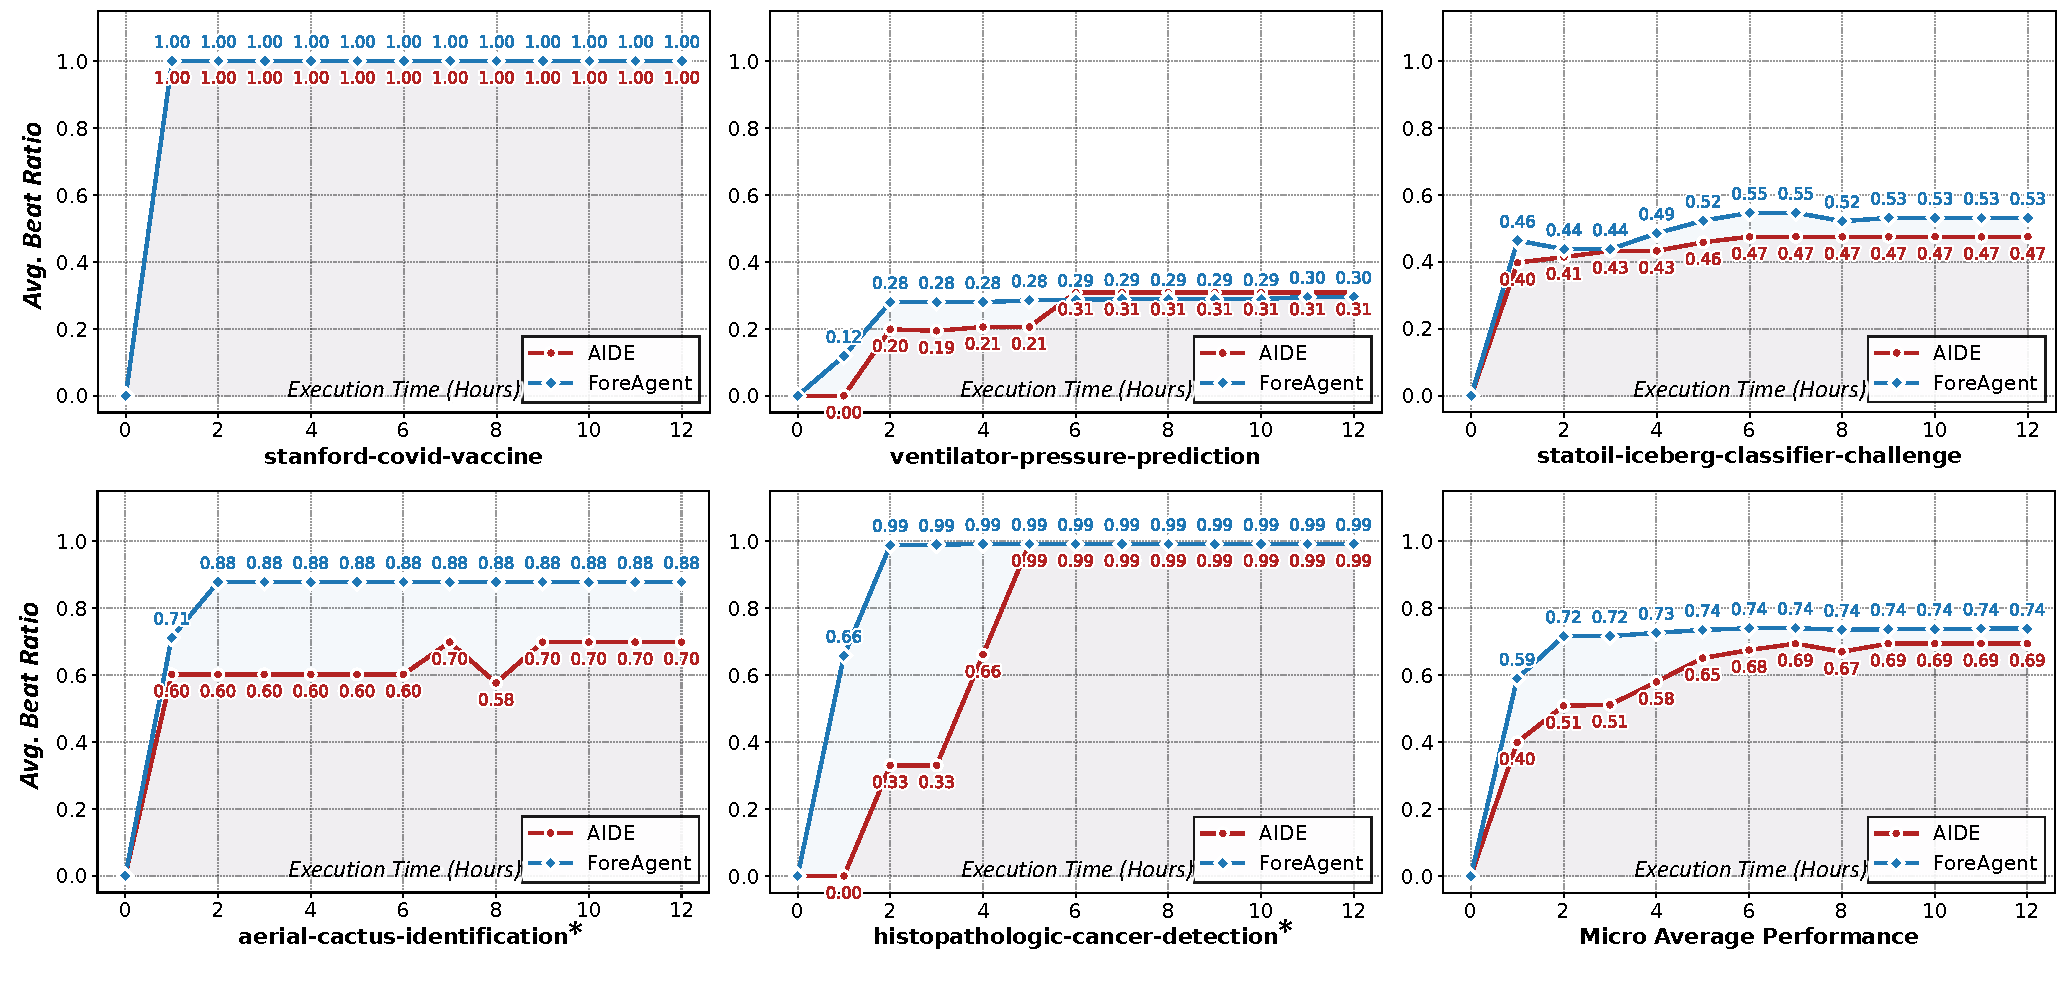
\includegraphics[width=\linewidth]{figures/appendix_agent_perf.pdf}
    \caption{\textbf{Temporal Evolution of Performance.} The curves display the Average Beat Ratio as a function of Execution Time (0--12 hours) for both the AIDE baseline and \textsc{ForeAgent}. The results are broken down by the five individual AI4Science tasks and the overall Micro Average.}
    \label{fig:appendix_agent_perf}
\end{figure*}

\begin{figure*}
    \centering
    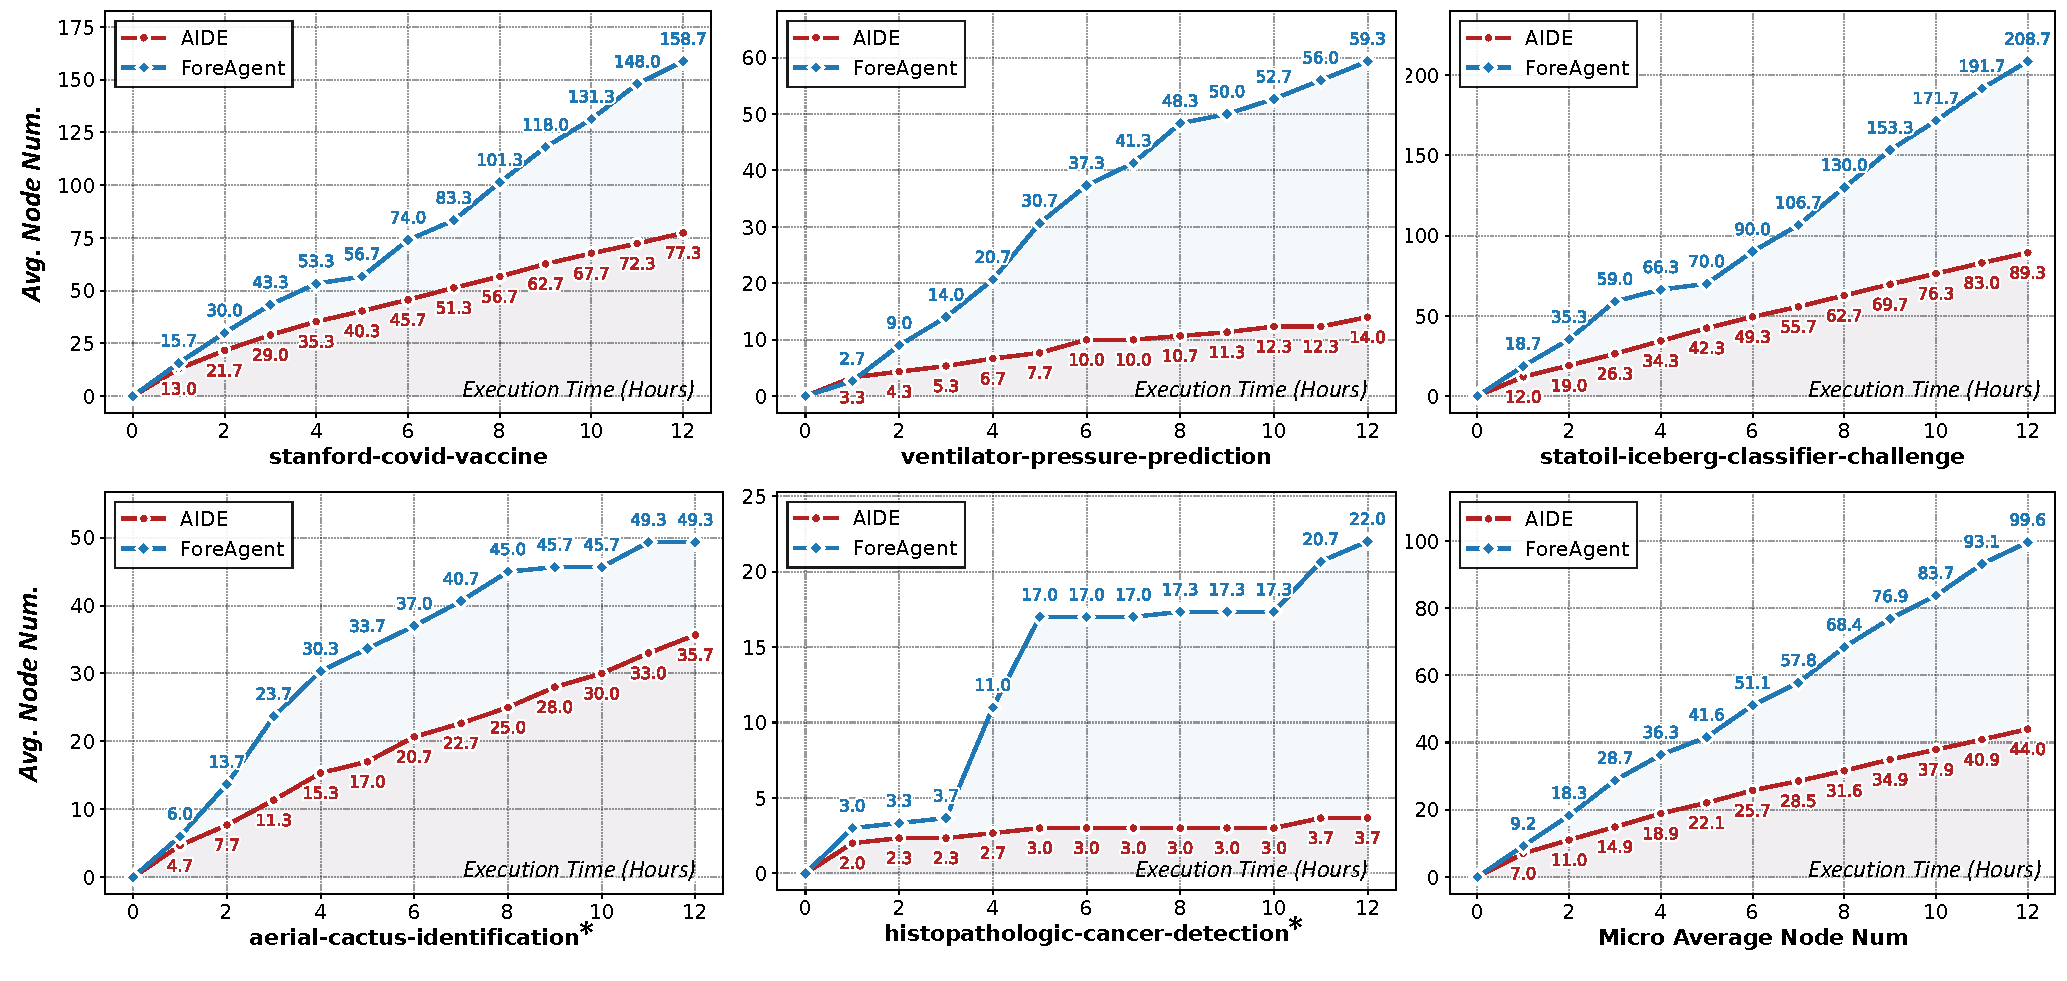
\includegraphics[width=\linewidth]{figures/appendix_agent_node.pdf}
    \caption{\textbf{Progression of Search Node Exploration.} This figure illustrates the cumulative number of nodes explored (Avg. Node Num.) over the 12-hour duration. It compares the search trajectories of \textsc{ForeAgent} against AIDE across each specific task and the aggregated Micro Average.}
    \label{fig:appendix_agent_node}
\end{figure*}

\begin{figure*}
    \centering
    % 请确保把文件名替换成你实际的文件名
    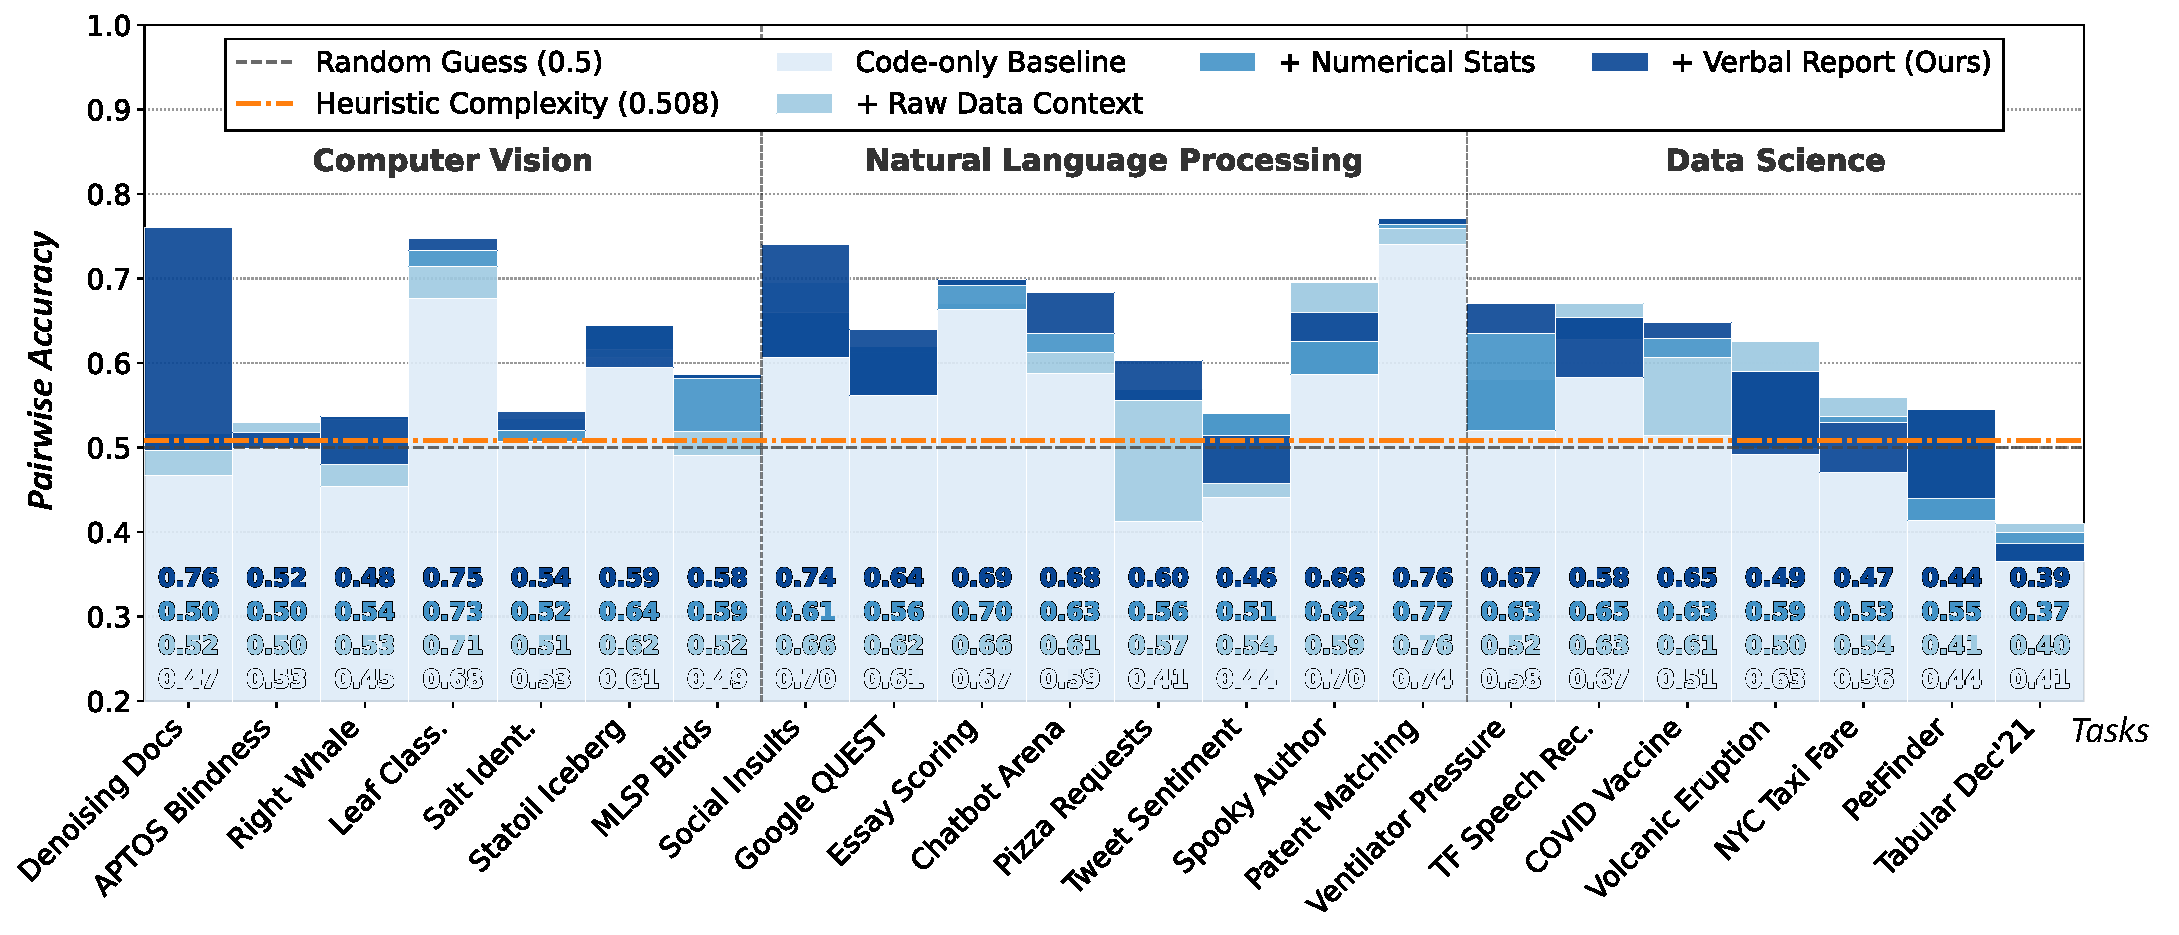
\includegraphics[width=\linewidth]{figures/appendix_data_repr.pdf}
    
    \caption{\textbf{Domain and Task Sensitivity Analysis.} The stacked bar chart presents the data representation study for each individual task. It visualizes the incremental performance impact of adding Raw Data, Numerical Statistics, and Verbal Reports to the Code-only baseline. The tasks are grouped by their respective domains (CV, NLP, and Data Science) to highlight domain-specific sensitivity.}
    \label{fig:appendix_domain_sensitivity}
\end{figure*}

% \clearpage


\section{Detailed Qualitative Analysis}
\label{appendix:case_studies}

% 引入包含所有四个Figure的文件
\begin{figure*}
    \centering
    
    % 调用外层框架
    \begin{CaseStudyFrame}{Case Study: Human Intuition v.s. World Model Inference}{fig:case_study_quest}
        
        % 1. 上下文
        \ContextBar{
            \textbf{Task:} Google Quest Challenge (Multi-label Subjective QA Regression). \\
            \textbf{Data Profile:} Small scale ($N_{train} \approx 5.5k$) with 30 \textit{heavily discretized} and \textit{skewed} targets. \\
            \textbf{Data Report Insight:} Strong Question-Group structure (85\% of target variance is explained by Q-means) creates high \textbf{Leakage Risk} in random splits.
        }
        
        % 2. 左右分栏结构
        % --- 左栏：Solution 0 (Deep Learning) ---
        \begin{minipage}[t]{0.49\linewidth}
            \begin{SolutionColumn}{myblue!50!black!80}{red!10}{Solution 0: Deep Learning w/ Cross-Attention}{A}
                \small % 整体字体变大
                % Stack 去掉 texttt，使用默认字体
                \textbf{Stack:} SentenceTransformer + MultiHead-CrossAttn + AdamW \\
                \textbf{Setup:} Holdout Validation (Random Split), MSE Loss.
                \par\vspace{2pt}
                \textbf{Actual Score:} \textcolor{red!60!black}{\textbf{0.2961} \ding{116}} (Spearman $\rho$)
                
                \vspace{0.2cm} \hrule \vspace{0.2cm}
                
                % Human View (Gray)
                % Human 预测它是 Favorite (赢)，实际输了 -> 错误 (Cross)
                \HumanView{Neural Network with Cross-Attention explicitly models QA interaction. Pre-trained embeddings capture superior semantics compared to statistical features.}{Strong Favorite \textcolor{red}{\faTimes}}
                \vspace{-2pt}
                
                % WM View (Blue)
                % WM 批评它有过拟合风险 (输)，实际输了 -> 正确 (Check)
                \WMView{Critique}{Model is underconstrained for small data ($5.5k$). Random split ignores question groups, causing leakage. High overfitting risk.}{Overfitting Risk \textcolor{green!60!black}{\faCheck}}
            \end{SolutionColumn}
        \end{minipage}%
        \hfill
        % --- 右栏：Solution 1 (LightGBM) ---
        \begin{minipage}[t]{0.49\linewidth}
            \begin{SolutionColumn}{myblue!50!black!80}{green!10}{Solution 1: LightGBM Ensemble}{A}
                \small % 整体字体变大
                % Stack 去掉 texttt
                \textbf{Stack:} TF-IDF + TruncatedSVD + LightGBM \\
                \textbf{Setup:} 5-Fold Cross Validation + Weighted Ensemble Optimization.
                \par\vspace{2pt}
                \textbf{Actual Score:} \textcolor{green!40!black}{\textbf{0.3145} \ding{115}} (Spearman $\rho$)
                
                \vspace{0.2cm} \hrule \vspace{0.2cm}
                
                % Human View (Gray)
                % Human 认为它是 Weak (输)，实际赢了 -> 错误 (Cross)
                \HumanView{TF-IDF is outdated. LightGBM is typically for tabular data, not text. The method is too simple, likely to underfit complex modern natural language processing tasks.}{Weak Baseline \textcolor{red}{\faTimes}}
                \vspace{-2pt}
                
                % WM View (Blue)
                % WM 认为它是 Optimal (赢)，实际赢了 -> 正确 (Check)
                \WMView{Insight}{Robust choice. 5-Fold CV provides honest estimates. SVD captures global label families. Sample-efficient given data scarcity.}{Optimal Fit \textcolor{green!60!black}{\faCheck}}
            \end{SolutionColumn}
        \end{minipage}
        
        % 3. 底部总结
        \OutcomeFooter{Solution 1 outperformed Solution 0. The World Model correctly prioritized \textbf{Validation Rigor} and \textbf{Sample Efficiency} over Architectural Sophistication.}
        
    \end{CaseStudyFrame}
    
    \caption{\textbf{Case Study: Human Intuition vs. World Model Inference.} This example illustrates a \textbf{hidden logical conflict} where architectural sophistication (favored by humans) clashes with data constraints. By leveraging the generated \textbf{Data Report}, the World Model detects a critical mismatch between the small dataset size ($N \approx 5.5k$) and the complex neural network (Solution 0). It correctly prioritizes the robust LightGBM ensemble (Solution 1), demonstrating the ability to weigh \textit{Data-Model Fit} over pure algorithmic complexity.}

    \label{fig:case_study_quest}
\end{figure*}





\begin{figure*}[b]
    \centering
    
    % 调用外层框架
    \begin{CaseStudyFrame}{Case Study: Prioritizing Domain Fit over SOTA Architecture}{fig:case_study_tgs}
        
        % 1. 上下文
        \ContextBar{
            \textbf{Task:} TGS Salt Identification (Pixel-level Segmentation). \\
            \textbf{Data Profile:} Small scale ($101 \times 101$) grayscale seismic images with weak intensity contrast and high variability in mask coverage. \\
            \textbf{Data Report Insight:} High sensitivity to spatial artifacts; resizing introduces interpolation noise that destroys local salt boundary details. Depth data is unavailable (NaN).
        }
        
        % 2. 左右分栏结构
        % --- 左栏：Solution 0 (ViT) ---
        \begin{minipage}[t]{0.49\linewidth}
            \begin{SolutionColumn}{myblue!50!black!80}{red!10}{Solution 0: Vision Transformer}{A}
                \small
                \textbf{Stack:} ViT-B/16 (Pre-trained on ImageNet) \\
                \textbf{Setup:} Resize to $224 \times 224$, BCE + Dice Loss, attempts to use depth channel.
                \par\vspace{2pt}
                \textbf{Actual Score:} \textcolor{red!60!black}{\textbf{0.1301} \ding{116}} (mAP)
                
                \vspace{0.2cm} \hrule \vspace{0.2cm}
                
                % Human View (Gray)
                \HumanView{ViT is a top-tier SOTA model offering global context modeling. Pre-training on ImageNet guarantees strong feature extraction capabilities.}{Strong Favorite \textcolor{red}{\faTimes}}
                \vspace{-2pt}
                
                % WM View (Blue)
                \WMView{Critique}{Resizing $101 \times 101$ inputs to $224 \times 224$ risks losing fine details. Domain gap between ImageNet (RGB) and seismic data (grayscale) is severe. Incorrectly relies on missing depth data.}{Resolution Mismatch \textcolor{green!60!black}{\faCheck}}
            \end{SolutionColumn}
        \end{minipage}%
        \hfill
        % --- 右栏：Solution 1 (U-Net) ---
        \begin{minipage}[t]{0.49\linewidth}
            \begin{SolutionColumn}{myblue!50!black!80}{green!10}{Solution 1: Standard U-Net}{A}
                \small
                \textbf{Stack:} Custom U-Net with Hybrid Attention \\
                \textbf{Setup:} Native $101 \times 101$ resolution, BCE Loss, Test Time Augmentation (TTA).
                \par\vspace{2pt}
                \textbf{Actual Score:} \textcolor{green!40!black}{\textbf{0.6396} \ding{115}} (mAP)
                
                \vspace{0.2cm} \hrule \vspace{0.2cm}
                
                % Human View (Gray)
                \HumanView{Standard U-Net is an older, basic baseline. It lacks the global receptive field and advanced attention mechanisms of modern transformers.}{Weak Baseline \textcolor{red}{\faTimes}}
                \vspace{-2pt}
                
                % WM View (Blue)
                \WMView{Insight}{Preserves native spatial resolution without interpolation noise. Attention mechanisms efficiently capture multi-scale features and spatial dependencies crucial for weak-contrast segmentation.}{Optimal Fit \textcolor{green!60!black}{\faCheck}}
            \end{SolutionColumn}
        \end{minipage}
        
        % 3. 底部总结
        \OutcomeFooter{Solution 1 outperformed Solution 0. The World Model was not swayed by the ``SOTA'' status, correctly prioritizing \textbf{Native Spatial Resolution} and \textbf{Domain Fit} over superficial architectural complexity.}
        
    \end{CaseStudyFrame}
    
    \caption{\textbf{Case Study: Domain Fit vs. Architectural Sophistication.} This example highlights a ``square peg in a round hole'' scenario. While human intuition might favor the SOTA Vision Transformer (Solution 0), the World Model detects that forcing small $101 \times 101$ seismic images into ViT's required resolution introduces destructive interpolation noise. It rejects the complex model in favor of a U-Net (Solution 1) that preserves native spatial details and avoids relying on missing depth data, demonstrating skepticism towards superficially sophisticated but methodologically flawed approaches.}
    \label{fig:case_study_tgs}
\end{figure*}




\begin{figure*}
    \centering

\begin{ReportFrame}{Case Study: Verbal Data Report ($D_{rep}$) Sample for Task ``US Patent Matching''}{fig:long_report_content_1}

\#\# Data Overview

Train: 32,825 pairs; Test: 3,648 pairs. Columns: id, anchor... score (train only; in \{0.0... 1.0\}). No missing values...

106 unique 4-character CPC contexts; coverage across major sections... broad and similar in train/test.

Anchors: 733 unique; heavily reused (mean \textasciitilde 45 pairs per anchor...). Targets: 26,850 unique...

Test anchors: 100\% seen... Test targets: \textasciitilde 29\% seen... Test OOV rate \textasciitilde 12.5\%.
\newline

Why this structure matters:

The evaluation setting is anchor-centric... rewards learning anchor-specific decision boundaries and context-conditioned mappings...
\newline

\#\# Key Statistical Findings

Discrete labels concentrated at 0.25 and 0.5... Implication: strong class imbalance toward moderate similarity...

Correlation with score: char 3-5gram TF-IDF cosine \textasciitilde 0.46... Implication: surface overlap explains much variance but not all...

Phrases are very short (mean \textasciitilde 2 tokens...)... Implication: models will rely on token/subword and character patterns...

Context means vary... Implication: the mapping from lexical similarity to score is context-dependent...

Anchors average \textasciitilde 45 target pairs... Implication: each anchor induces a nontrivial local decision boundary...

Distributions are stable... Implication: generalization hinges on handling unseen targets...
\newline

\#\# Implications for Model Design

(Linking observation → modeling implication → evaluation impact)

Loss functions that ignore ordinality may mis-penalize near misses... Rank-sensitive metrics will reward monotonic mappings...

Architectures emphasizing character/subword patterns... align with dominant signal... Performance differences will emerge in tail cases...

Pairwise encoders that allow rich anchor-target interactions can learn... Approaches that exploit anchor identity will likely score well...

Models benefit from mechanisms that allow interaction between context and similarity features... Per-context performance may vary...

High-capacity sequence models may be underutilized on such short inputs... Efficiency-capacity trade-offs skew toward models effective on short spans...

Representations that degrade gracefully on unseen words... have an advantage... Robust handling of OOV will particularly improve performance...

Simple identity detection captures some easy gains... however, near-identical forms can still have scores <1.0...

Character CNNs... Token-level transformers... Independent encoders... Joint encoders... Denoising pretraining...
\newline

\#\# Summary

The dataset is anchor-centric... Surface-form similarity explains a large portion... Evaluation emphasizes generalization to new targets...

Capture strong character/subword overlap signals... Maintain robustness to unseen target tokens... Avoid over-reliance on identity heuristics... Account for label ordinality...
    
\end{ReportFrame}
    
\captionof{figure}{\textbf{Case Study: Verbal Data Report ($D_{rep}$) Sample for ``US Patent Matching''.} Generated via the \textit{Code-Execution-Verbalization} protocol, this artifact bridges the gap between raw data statistics and semantic reasoning.}
\label{fig:report_patent}

\end{figure*}




\begin{figure*}
    \centering

\begin{ReportFrame}{Case Study: Task Instruction ($I$) for Task ``Denoising Dirty Docs''}{fig:long_report_content_0}

\# Overview

\#\# Description

Optical Character Recognition (OCR) is the process of converting typed or handwritten documents into a digitized format. OCR makes previously static content editable, searchable, and easier to share.

This task focuses on improving OCR performance for degraded scanned documents. Given a dataset of noisy text images, the goal is to develop a model that removes visual noise such as stains, fading, and wrinkles, producing cleaner text images suitable for further processing and digitization.

\#\# Evaluation

Submissions are evaluated using the root mean squared error (RMSE) between the predicted cleaned pixel intensities and the ground truth grayscale pixel intensities.

\#\#\# Submission Format

Each image is represented as a list of pixel values with identifiers in the form 'image\_row\_col' (e.g. '1\_2\_1' for image 1, row 2, column 1). Intensity values range from 0 (black) to 1 (white).

\verb|```|

id,value
1\_1\_1,1
1\_2\_1,1
1\_3\_1,1
...

\verb|```|

\#\# Data

\#\#\# Dataset Description

The dataset contains two sets of images: 'train' and 'test'.  
- The 'train' set includes noisy text images and their corresponding cleaned versions ('train\_cleaned').
- The 'test' set contains only noisy images that need to be denoised.

The noise simulates real-world artifacts commonly seen in scanned documents, such as blur, stains, and faded ink. The task is to build a model that restores the test images to a clean, readable form.

\#\#\# File Description

- There are three directory corresponding to the data description above: 'train', 'train\_cleaned' and 'test'.
- The sample submission is stored in sampleSubmission.csv.
    
\end{ReportFrame}
    
\captionof{figure}{\textbf{Case Study: Task Instruction ($I$) for Task ``Denoising Dirty Docs''.} 
This example illustrates the raw natural language input $I$ as defined in Section~\ref{sec:agent_paradigm}. 
It outlines the problem context, dataset specifications, and evaluation criteria, serving as the foundational prompt that initiates the agent's solution generation process.}
\label{fig:task_instruction_denoising}

\end{figure*}

To validate the model's reasoning depth and provide transparency into our pipeline, we present four qualitative examples.
First, we analyze two reasoning trajectories (Google Quest Challenge and TGS Salt Identification) to illustrate how the model acts as a skeptical critic, prioritizing methodological fit over superficial sophistication and overcoming human bias (Finding 5).
Subsequently, we provide visual samples of two critical system artifacts: the \textit{Verbal Data Report} and the \textit{Task Instruction}, enabling a concrete inspection of the agent's input and context.

\subsection{Case I: Overcoming Complexity Bias (Reasoning Analysis)}
\label{app:case_bias}

To provide a concrete example of Finding 5 (``The World Model Transcends Human Intuition by Prioritizing Data-Grounded Constraints''), we present a detailed analysis in Figure~\ref{fig:case_study_quest}.
This case illustrates a common pitfall where architectural sophistication clashes with fundamental data constraints.

\paragraph{Scenario and Conflict.}
The agent evaluates two distinct solutions for the Google Quest Q\&A task:
\begin{itemize}
    \item \textbf{Solution 0:} A complex Deep Neural Network (DNN) with Cross-Attention.
    \item \textbf{Solution 1:} A robust LightGBM ensemble.
\end{itemize}
Intuitively, human evaluators and models relying solely on code complexity heuristics often exhibit a ``complexity bias'' by favoring the deep learning approach under the assumption that greater architectural depth yields better performance.

\paragraph{World Model Reasoning.}
However, the World Model leverages the generated Data Analysis Report to detect a critical mismatch.
The report highlights that the dataset is relatively small ($N \approx 5.5k$ samples) with skewed targets.
Synthesizing this finding with model design principles, the World Model predicts a high risk of overfitting for the complex DNN.
Consequently, it correctly prioritizes the LightGBM ensemble (Solution 1), determining that the gradient boosting approach offers a superior Data-Model Fit for this specific sample size.

\subsection{Case II: Domain Fit over Architectural Sophistication}
\label{app:case_domain}

To further substantiate the model's robustness against complex-looking but flawed solutions (``Square peg in a round hole''), we present a second trajectory analysis in Figure~\ref{fig:case_study_tgs}.

\paragraph{Scenario and Conflict.}
The agent evaluates two segmentation solutions for the TGS Salt Identification task:
\begin{itemize}
    \item \textbf{Solution 0:} A Vision Transformer (ViT-B/16) pre-trained on ImageNet.
    \item \textbf{Solution 1:} A standard U-Net.
\end{itemize}
Human intuition might favor the ViT due to its top-tier status and global context modeling capabilities.

\paragraph{World Model Reasoning.}
The World Model recognizes that the task requires pixel-perfect segmentation of small ($101 \times 101$) seismic images. It correctly identifies that forcing inputs into the ViT's required $224 \times 224$ resolution introduces interpolation noise and destroys fine-grained salt details. Unswayed by the ``SOTA'' status, the model rejects the ViT in favor of the standard U-Net, citing the necessity of preserving native spatial resolution and avoiding severe domain mismatch.

\subsection{Case III: Sample of the Verbal Data Report}
\label{app:case_report}

Figure~\ref{fig:report_patent} presents a representative sample of the Verbal Data Report ($D_{rep}$) generated for the \textit{US Patent Matching} task.
This artifact visualizes the mechanism described in Section~\ref{sec:input_augmentation}: transforming raw execution logs (e.g., text length statistics, label skew) into semantic narratives.
It serves as the grounding anchor that allows the language model to ``read'' and internalize dataset properties without direct access to the raw files.

\subsection{Case IV: Sample of the Task Instruction ($I$)}
\label{app:case_instruction}

Finally, to visualize the input definition provided in Section~\ref{sec:agent_paradigm}, Figure~\ref{fig:task_instruction_denoising} displays the raw Task Instruction ($I$) for the task \textit{Denoising Dirty Docs}.
This prompt encapsulates the natural language description, specific dataset paths, and optimization goals, acting as the initial state that triggers the agent's autonomous loop.


\section{Prompt Templates}
\label{appendix:prompt_templates}

To ensure reproducibility and transparency, we provide the full prompt templates used in our World Model framework. The workflow consists of four key stages:

\begin{enumerate}
    \item \textbf{Data Analysis Code Generation (Figure~\ref{fig:appendix_da_code_prompt}):} The agent is first instructed to generate a robust Python script for profiling the dataset. This step extracts key statistical meta-features without training a model.
    \item \textbf{Data Analysis Report Generation (Figure~\ref{fig:appendix_da_report_prompt}):} Based on the execution logs from the previous step, the agent summarizes the findings into a structured, causal report. This report serves as a critical context for the reasoning engine.
    \item \textbf{Result Prediction Query (Figure~\ref{fig:appendix_result_predict_query}):} This is the core reasoning prompt where the World Model predicts the relative performance of candidate solutions. It integrates the task description, the generated data analysis report, and the solution code to form a grounded judgment.
    \item \textbf{Complexity Scoring (Figure~\ref{fig:appendix_complexity_prompt}):} An auxiliary prompt used to calculate the complexity heuristic baseline. It evaluates solutions across code engineering, model architecture, and data pipeline dimensions to detect potential bias towards complexity.
\end{enumerate}

The specific prompt templates are illustrated below.


\onecolumn
% 引入外部的 Prompts 文件
\begin{promptbox}{Prompt: Data Analysis Code Generation}
\textbf{SYSTEM:} 

You are an expert Data Science Architect specializing in automated dataset profiling and meta-learning. Your goal is to write a robust, error-handling Python script that extracts high-level statistical and structural insights from a dataset without performing full model training.
\newline

\textbf{USER:}

I need you to generate a Python script to analyze a dataset for the following machine learning task.

Context:

Task Description: \textbf{\{task-desc\}}

Data Directory: \textbf{\{data-dir\}}

Requirements for the Python Script:

Data Loading \& Robustness:
The script must determine the correct data type (Tabular, CV, NLP, or Time-Series) based on the Task Description and file extensions in {data-dir}.
Implement strictly robust file loading (e.g., using try-except blocks). If files are too large, perform stratified sampling (load max 10k rows or 1000 images).

Key Metric Extraction (Crucial for World Model Prediction):
Do not just print raw data. Calculate and print meta-features that correlate with model difficulty.

Output Format:
The script must print the analysis results to stdout in a structured, human-readable text format (or JSON structure) that a downstream LLM can easily parse to write a report.
Do not generate plots/images. Only generate text logs/stats.

Constraints:
Use only standard libraries: pandas, numpy, scipy, sklearn, PIL (for images), os, glob.
Do not attempt to train any machine learning models (e.g., do not run Random Forest).

Response: Provide only the executable Python code block.
\end{promptbox}
 % --- End of Prompt Box ---

\captionof{figure}{Prompt used to instruct the LLM for generating data analysis code.} % 图注
\label{fig:appendix_da_code_prompt} % <--- 这里的 label 用于后续引用


\vspace{2em}


\begin{promptbox}{Prompt: Data Analysis Report Generation}

You are preparing a structured Data Analysis Report that will be provided to another expert LLM. Your goal is to make the data characteristics and their implications explicit, causal, and model-relevant — so that a model evaluation agent can reason about how the dataset properties interact with model design choices.
\newline

Follow these instructions carefully:

1. Summarize, don’t just restate numbers.

    - Extract key quantitative trends (e.g., mean intensity, noise variability, contrast, etc.).

    - Highlight patterns, anomalies, and dataset biases.

2. Establish causal implications for modeling.

    - For each key observation, explain why it matters for model training, architecture, or generalization.
    
    - Example: “High inter-sample heterogeneity suggests the model should include normalization or data augmentation to handle distribution shift.”

3. Bridge data to model choices.

    - Express potential advantages or risks for different architectures (CNNs, transformers, denoising autoencoders, etc.) given the observed data patterns.
    
    - DONT directly suggest which model / method is better. You only need to analyze the potential advantages or risks.

4. Directly suggesting models will strongly result in bias.

    - DONT directly suggest which model / method is better. You only need to analyze the potential advantages or risks.

5. Maintain a clear structure using the following format:
\begin{verbatim}
## Data Overview
    <summary of dataset structure, splits, file composition>

## Key Statistical Findings
<highlighted numeric findings + what they imply>

## Implications for Model Design
    <how these data patterns affect likely model performance>

## Summary
    <concise conclusion connecting data traits to modeling priorities>
\end{verbatim}

6. Tone and length:

    - Write concisely and analytically (like a scientific data report).
    
    - Do not include raw metrics dumps.
    
    - Focus on interpretability and causal reasoning.
\newline

Your output will serve as the \{<data\_analysis>\} section for a reasoning-based model evaluator.
Ensure every insight has a clear link from data observation $\to$ modeling implication $\to$ evaluation impact.

INPUT CONTEXT:

[Task Name]
\textbf{\{task\}}

[Task Description]
\textbf{\{desc-block\}}

[Raw Data Analysis Extraction]
\textbf{\{analysis-text\}}
\newline

RESPONSE: Produce the final structured report now. Follow the required headings exactly. Avoid recommending specific models; only analyze potential advantages or risks.
\end{promptbox}
% --- End of Prompt Box ---
\caption{Prompt used to instruct the LLM for generating data analysis report from the code execution result.} % 图注
\label{fig:appendix_da_report_prompt} % <--- 这里的 label 用于后续引用


\vspace{2em}


\begin{promptbox}{Prompt: Result Prediction Query}
     
\textbf{SYSTEM:}

You are an ML code and data analysis expert tasked with predicting the relative performance of provided ML solutions without executing any code. Base your judgment on the task description and the shown code snippets only. Never assume external ground-truth. You should include brief reasoning before the final answer. End your answer with a single JSON object that strictly matches the specified response format.
\newline

\textbf{USER:}

Task: 

\textbf{\{task-name\}}

Task description:

\textbf{\{task-desc\}}

Data analysis:

\textbf{\{data-analysis-report\}}
\newline

Important instructions:

- Predict which solution will perform best (or provide a full ranking) WITHOUT running code.

- Use only the task description, data analysis, and code snippets below.

- Treat the task description and data analysis as equally important to the code; analyze them separately, surface their underlying implications, and provide a balanced, trade-off judgment. 

- Connect data analysis to the following code analysis: If data analysis indicates properties , explain how the architecture addresses them , forming a data→why→method choice causal chain.

- Forbid the “complexity-wins” shortcut: Do not claim “deeper/more complex/with attention is better” as the sole reason. If used, justify why it holds under the current data distribution and training details, and provide a counterexample scenario.

- Response format: \{"predicted\_best\_index": <0 or 1>, "confidence": <optional float>\}

- Indices correspond to the order of the listed solutions (0..n-1).

- You should include brief reasoning before the final JSON. End with a single JSON object matching the response format. Do not write anything after the JSON.
\newline

Provided solutions:

Solution 0: path=\textbf{\{code-0-path\}}

\textbf{\{code-snippet-0\}}

Solution 1: path=\textbf{\{code-1-path\}}

\textbf{\{code-snippet-1\}}

\end{promptbox}
% --- End of Prompt Box ---
\caption{Prompt used to instruct the LLM for predicting the result of the provided materials.} % 图注
\label{fig:appendix_result_predict_query} % <--- 这里的 label 用于后续引用


\vspace{2em}


\begin{promptbox}{Prompt: Complexity Scoring Query}
    
\textbf{SYSTEM:}

You are an expert Machine Learning Engineer and Researcher.
Your task is to analyze a Python script for a machine learning task and evaluate its complexity based on three specific dimensions.

You must output a JSON object with three scores (integers from 1 to 10) and a brief reasoning for each.
\newline

The dimensions are:

1. code\_engineering\_score (1-10): Cyclomatic complexity, custom logic, dependence depth, messy custom loops vs clean API calls.

2. model\_arch\_score (1-10): Parameter count, FLOPs, depth of network, novelty of architecture (e.g., Transformer > Simple CNN).

3. data\_pipeline\_score (1-10): Complexity of preprocessing, data augmentation strategies (Mixup, TTA), custom sampling logic.
\newline

Output Format:

\texttt{\{}

\hspace{1em} "code\_engineering\_score": <int>,

\hspace{1em} "model\_arch\_score": <int>,

\hspace{1em} "data\_pipeline\_score": <int>,

\hspace{1em} "reasoning": "<short summary>"

\texttt{\}}
\newline

\textbf{USER:}

Analyze the following Machine Learning code and provide complexity scores.

\textbf{\{code\_snippet\}}

Respond ONLY with the valid JSON.

\end{promptbox}
% --- End of Prompt Box ---
\caption{Prompt used to instruct the auxiliary LLM for scoring the complexity of code solutions across three dimensions. This heuristic is used as a baseline to evaluate whether the World Model blindly favors complex code.}
\label{fig:appendix_complexity_prompt}


% \clearpage





% 更多的讨论
% 为什么coder模型没有更好
% 为什么中等难度的任务打得最好